\documentclass[10pt,a4paper]{article}
\usepackage[margin=2.1cm]{geometry}
\usepackage{fontspec,unicode-math}
\setmainfont{Libertinus Serif}\setsansfont{IBM Plex Sans}[Scale=0.9]\setmonofont{IBM Plex Mono}[Scale=0.82]
\setmathfont{Libertinus Math}
\usepackage{graphicx,booktabs,tabularx,multicol,xcolor,hyperref,enumitem,array}
\hypersetup{colorlinks,linkcolor=black,urlcolor=blue!50!black}
\newcommand{\ax}[1]{\par{\raggedright\noindent\hangindent=2.5em\hangafter=1 $#1$\par}\smallskip}
\setlength{\parindent}{0pt}\setlength{\parskip}{3pt}\setlength{\emergencystretch}{3em}
\title{A conceptual framework for biomedical experiments\\[2pt]\large and its OWL~2~DL axiomatization, classified by a reasoner}
\author{Generated by \texttt{rsa/experiment\_ontology.py}; all values ILLUSTRATIVE (D016)}
\date{}
\begin{document}\maketitle

\part*{I\quad A conceptual framework for biomedical experiments}
\section*{Core idea}
\emph{An experiment is a planned process that intervenes on and observes a biological system, executing a design, in
order to change a belief about hypotheses.} The framework keeps apart what is \emph{planned} (design, protocol), what
\emph{happens} (execution), what is \emph{measured} (data) and what is \emph{believed} (hypotheses, belief,
conclusions); the biology is the hidden state in between, reached only through interventions and through readouts that
are proxies for it. No biological fact or parameter is asserted: hypotheses \emph{posit} biology, data are
\emph{proxies} (D016).

\begin{center}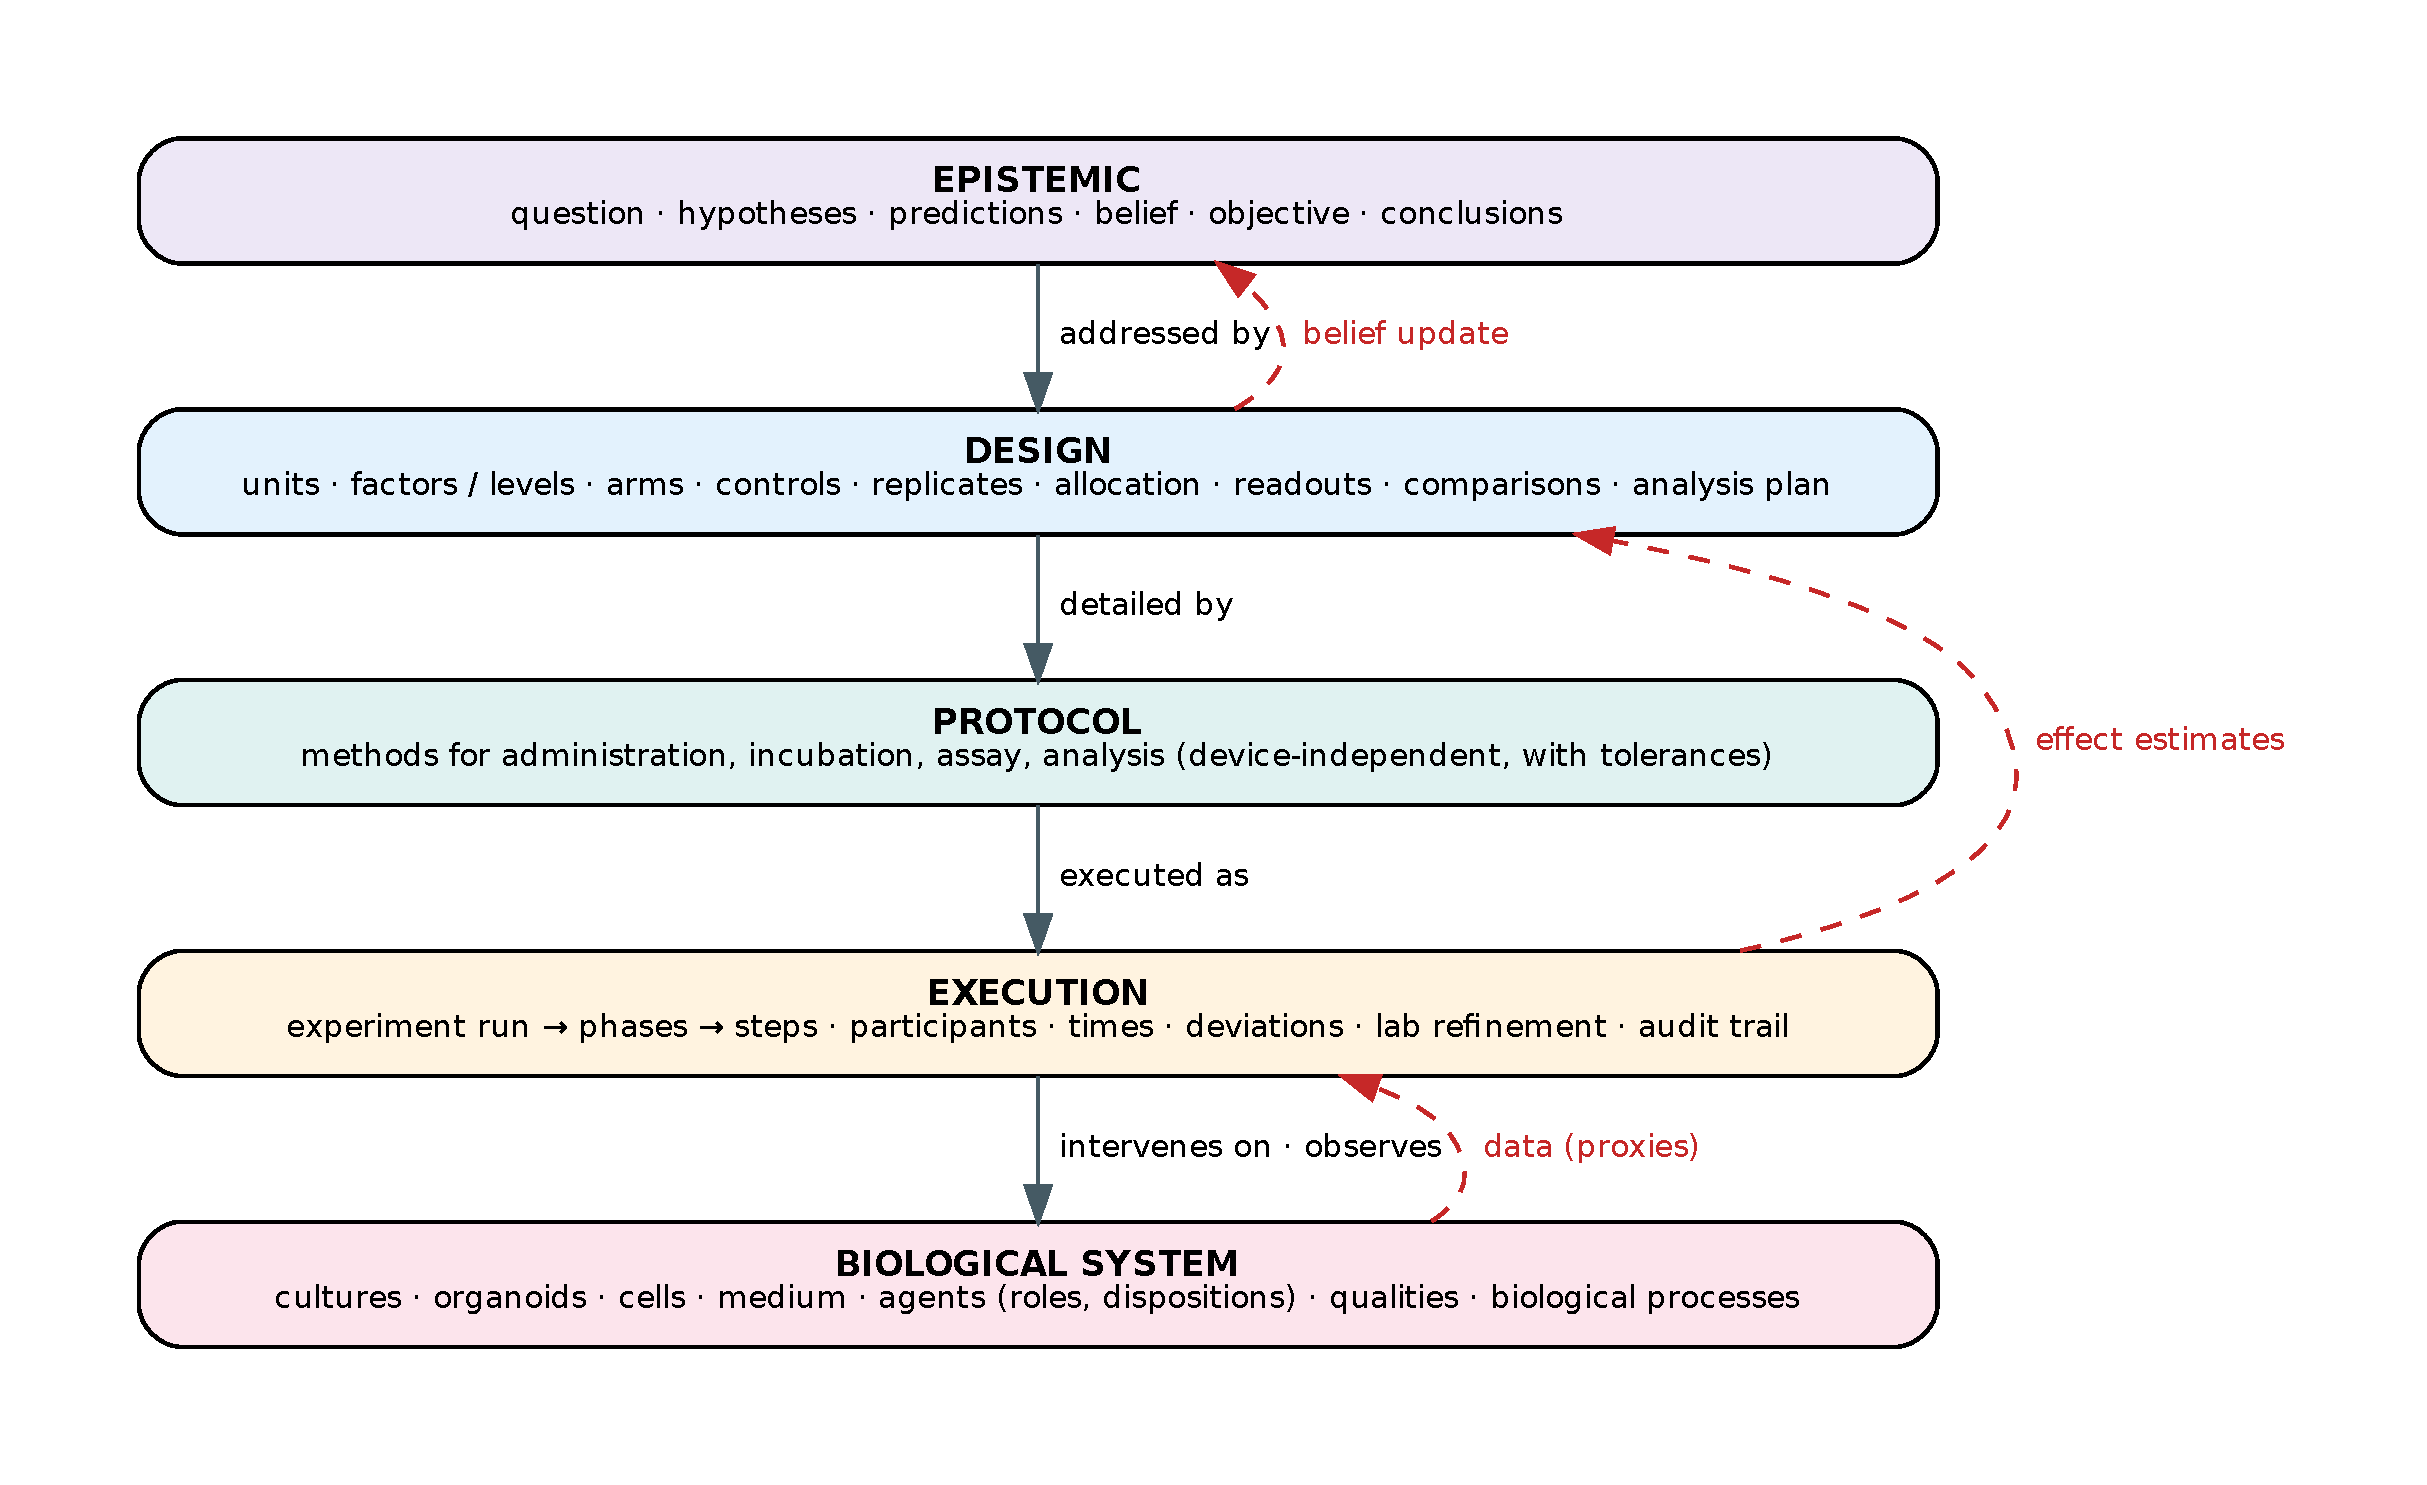
\includegraphics[width=0.92\linewidth]{framework.pdf}\end{center}

\section*{Core concepts}
{\small\begin{tabularx}{\linewidth}{@{}>{\raggedright\arraybackslash}p{3.1cm}>{\raggedright\arraybackslash}X@{}}\toprule
Experimental unit & what is treated independently and measured (a culture in a well) \\
Factor, level & what is varied (agent, dose, time of rescue) and the values it takes \\
Treatment & one combination of levels, given as a schedule of administrations \\
Arm & a treatment and the units assigned to it (membership, not parthood) \\
Control & an arm defined by what it controls for: negative (untreated, vehicle), positive (expected effect from prior
evidence), agent-alone (the agent's own effect), comparator (isolates one factor) \\
Replicate & units under the same treatment; biological (independent units) vs technical (repeated measurements) \\
Allocation & assignment and placement of units: randomisation, blocking, avoiding edge wells, blinding \\
Readout & the measured quantity, its time and assay, and what it is a proxy for (size for viability) \\
Comparison & a pair of arms whose difference estimates the effect of exactly one factor \\
Interaction contrast & a difference of comparisons: does a factor's effect depend on another factor \\
Validity check & a comparison that licenses another (injury happened; the agent works) \\
Analysis plan & the decision rule of every comparison and the handling of deviations, fixed before the run \\
Hypothesis, prediction & a model that posits processes, and its expected effect for a comparison \\
Belief, information gain & a probability over hypotheses, and how much a design is expected to change it \\
Deviation & a difference between execution and plan; it can invalidate comparisons \\
Conclusion (insight) & a statement derived from effect estimates and the posterior, with provenance \\
\bottomrule\end{tabularx}}

\section*{Taxonomy along independent axes}
System (in silico, in vitro, ex vivo, in vivo, clinical); purpose (exploratory, confirmatory, hypothesis-discriminating,
dose--response, time-course); design structure (comparative, controlled, factorial, within- or between-unit,
randomised, blinded); intervention (challenge, rescue or therapy, both); adequacy (validated, agent-controlled,
positive-controlled, replicated, pre-specified). Classes are \emph{defined}, so a reasoner places an experiment under
every class it satisfies (Part~II).

\section*{Criteria and how each is enforced}
{\small\begin{tabularx}{\linewidth}{@{}>{\raggedright\arraybackslash}p{2.2cm}>{\raggedright\arraybackslash}X>{\raggedright\arraybackslash}p{4.6cm}@{}}\toprule
validity & criteria & enforced by \\ \midrule
internal & single factor per comparison; negative, agent-alone and positive controls; randomisation; blinding & defined classes (reasoner); closed-world checks \\
statistical & biological replicates; expected information or power & closed-world counts; information-gain model \\
construct & readout states its proxy relation; manipulation checked (validity comparison) & ontology; licensing order in the plan \\
executional & identity, contamination, environment kept; plan realized; deviations recorded & run-time monitors (CRAM); audit trail \\
external & relevance of the system to the target biology & stated as an assumption, never inferred \\
\bottomrule\end{tabularx}}

\emph{Description logic for what experiments are; closed-world queries for what a design must contain; run-time monitors
for what an execution must keep; probabilistic models for what it will tell us.}

\section*{Lifecycle}
Question $\rightarrow$ hypotheses and predictions $\rightarrow$ candidate designs $\rightarrow$ selection (information vs
cost) $\rightarrow$ \textbf{adequacy check before the run} $\rightarrow$ protocol $\rightarrow$ refinement into lab actions
$\rightarrow$ monitored execution $\rightarrow$ data $\rightarrow$ analysis by the pre-specified rules $\rightarrow$ belief
update $\rightarrow$ conclusions $\rightarrow$ next question. Foundations: BFO-style upper level, OBI patterns (planned
process, study design, assay), Cell~01's biology ontology for the domain.

\part*{II\quad The axiomatization}

\section*{What Part II is}
The challenge-rescue experiment axiomatized as a biomedical experiment in $\mathcal{SROIQ}(\mathbf{D})$ (OWL~2~DL).
One source gives the DL notation below, an OWL ontology (\texttt{experiment.ofn}, \texttt{experiment.owl}) and the
input of the HermiT reasoner, which checks consistency, classifies the concepts and realizes the individuals.
Compared with the first axiomatization, the design is a \emph{plan} that the experiment executes; cultures are
\emph{units assigned to arms} (membership, not parthood); agents are chemical entities bearing \emph{roles} and
\emph{dispositions}; arms, comparisons, designs and experiments are \emph{defined} concepts that the reasoner
classifies from their content; the biomedical adequacy of a design is part of the hierarchy; hypotheses are
information entities that \emph{posit} processes, so nothing biological is asserted as fact; size is a
\emph{proxy} for viability. Concepts are set in $\mathsf{sans}$, roles in $\mathit{italics}$, individuals in
$\mathtt{mono}$.

\section{Upper level}A BFO-style upper level. Continuants (material entities, qualities, realizable entities, information content entities) and occurrents (processes) are disjoint; planned processes are distinct from biological processes.
\begin{multicols}{2}
\ax{\mathsf{MaterialEntity} ⊑ \mathsf{Continuant}}
\ax{\mathsf{SpecificallyDependentContinuant} ⊑ \mathsf{Continuant}}
\ax{\mathsf{Quality} ⊑ \mathsf{SpecificallyDependentContinuant}}
\ax{\mathsf{RealizableEntity} ⊑ \mathsf{SpecificallyDependentContinuant}}
\ax{\mathsf{InformationContentEntity} ⊑ \mathsf{Continuant}}
\ax{\mathsf{Process} ⊑ \mathsf{Occurrent}}
\ax{\mathsf{Continuant} ⊓\allowbreak \mathsf{Occurrent} ⊑ ⊥}
\ax{\mathrm{Disjoint}(\mathsf{MaterialEntity},\allowbreak \mathsf{SpecificallyDependentContinuant},\allowbreak \mathsf{InformationContentEntity})}
\ax{\mathsf{Quality} ⊓\allowbreak \mathsf{RealizableEntity} ⊑ ⊥}
\ax{\mathsf{Role} ⊑ \mathsf{RealizableEntity}}
\ax{\mathsf{Disposition} ⊑ \mathsf{RealizableEntity}}
\ax{\mathsf{Role} ⊓\allowbreak \mathsf{Disposition} ⊑ ⊥}
\ax{\mathsf{PlannedProcess} ⊑ \mathsf{Process}}
\ax{\mathsf{BiologicalProcess} ⊑ \mathsf{Process}}
\ax{\mathsf{PlannedProcess} ⊓\allowbreak \mathsf{BiologicalProcess} ⊑ ⊥}
\ax{\mathsf{PlanSpecification} ⊑ \mathsf{InformationContentEntity}}
\ax{\mathsf{DataItem} ⊑ \mathsf{InformationContentEntity}}
\ax{\mathsf{Hypothesis} ⊑ \mathsf{InformationContentEntity}}
\ax{\mathsf{Objective} ⊑ \mathsf{InformationContentEntity}}
\ax{\mathsf{Conclusion} ⊑ \mathsf{InformationContentEntity}}
\ax{\mathrm{Disjoint}(\mathsf{PlanSpecification},\allowbreak \mathsf{DataItem},\allowbreak \mathsf{Hypothesis},\allowbreak \mathsf{Objective},\allowbreak \mathsf{Conclusion})}
\end{multicols}
\section{Relations and partonomy}Parthood is transitive and kind-preserving: processes have processes as parts, material entities material entities, information entities information entities. Its kinds are simple sub-roles (so they may be counted). Location, membership, participation, execution and bearing are not parthood.
\begin{multicols}{2}
\ax{\mathrm{Trans}(\mathit{hasPart})}
\ax{\mathit{partOf} ≡ \mathit{hasPart}^{-}}
\ax{\mathit{hasPhase} ⊑ \mathit{hasPart}}
\ax{\mathit{hasStep} ⊑ \mathit{hasPart}}
\ax{\mathit{hasWell} ⊑ \mathit{hasPart}}
\ax{\mathit{hasOrganoid} ⊑ \mathit{hasPart}}
\ax{\mathit{hasCell} ⊑ \mathit{hasPart}}
\ax{\mathit{hasMedium} ⊑ \mathit{hasPart}}
\ax{\mathit{hasArm} ⊑ \mathit{hasPart}}
\ax{\mathit{hasComparisonSpec} ⊑ \mathit{hasPart}}
\ax{\mathit{hasAdministrationSpec} ⊑ \mathit{hasPart}}
\ax{\mathit{hasObjective} ⊑ \mathit{hasPart}}
\ax{\mathsf{Process} ⊑ ∀\mathit{hasPart}.\mathsf{Process}}
\ax{\mathsf{MaterialEntity} ⊑ ∀\mathit{hasPart}.\mathsf{MaterialEntity}}
\ax{\mathsf{InformationContentEntity} ⊑ ∀\mathit{hasPart}.\mathsf{InformationContentEntity}}
\ax{\mathit{containedIn} ≡ \mathit{contains}^{-}}
\ax{\mathit{containedIn} ∘ \mathit{partOf} ⊑ \mathit{locatedIn}}
\ax{\mathit{participatesIn} ≡ \mathit{hasParticipant}^{-}}
\ax{\mathit{hasPart} ∘ \mathit{hasParticipant} ⊑ \mathit{hasParticipant}}
\ax{\mathit{hasSpecifiedInput} ⊑ \mathit{hasParticipant}}
\ax{\mathit{inheresIn} ≡ \mathit{bearerOf}^{-}}
\ax{\mathrm{Func}(\mathit{inheresIn})}
\ax{\mathit{hasAssignedUnit} ≡ \mathit{assignedTo}^{-}}
\ax{\mathrm{Func}(\mathit{assignedTo})}
\ax{\mathrm{Func}(\mathit{usesAgent})}
\ax{\mathrm{Trans}(\mathit{precedes})}
\ax{∃\mathit{executes}.⊤ ⊑ \mathsf{PlannedProcess}}
\ax{⊤ ⊑ ∀\mathit{executes}.\mathsf{PlanSpecification}}
\ax{∃\mathit{isAbout}.⊤ ⊑ \mathsf{InformationContentEntity}}
\ax{∃\mathit{bearerOf}.⊤ ⊑ \mathsf{Continuant}}
\ax{⊤ ⊑ ∀\mathit{bearerOf}.\mathsf{SpecificallyDependentContinuant}}
\ax{∃\mathit{realizedIn}.⊤ ⊑ \mathsf{RealizableEntity}}
\ax{⊤ ⊑ ∀\mathit{realizedIn}.\mathsf{Process}}
\ax{\mathrm{Func}(\mathit{dose_au})}
\ax{\mathrm{Func}(\mathit{atTime_h})}
\ax{\mathrm{Func}(\mathit{fromTime_h})}
\ax{\mathrm{Func}(\mathit{toTime_h})}
\ax{\mathrm{Func}(\mathit{expectedInformationGain_bits})}
\ax{\mathrm{Func}(\mathit{radius_um})}
\ax{\mathrm{Func}(\mathit{wellRow})}
\ax{\mathrm{Func}(\mathit{wellColumn})}
\end{multicols}
\section{Biological material and labware}An organoid culture is organoids in medium; an organoid has cells. A well holds at most one culture; a culture is in a well, not part of it. Chemical agents bear roles in the experiment (challenge, rescue, vehicle) and dispositions (toxicity); size is a quality of organoids, viability and recovery capacity are dispositions of cultures.
\ax{\mathsf{OrganoidCulture} ⊑ \mathsf{MaterialEntity} ⊓\allowbreak ∃\mathit{hasOrganoid}.\mathsf{Organoid} ⊓\allowbreak ∃\mathit{hasMedium}.\mathsf{CultureMedium}}
\ax{\mathsf{Organoid} ⊑ \mathsf{MaterialEntity} ⊓\allowbreak ∃\mathit{hasCell}.\mathsf{Cell}}
\ax{\mathsf{Cell} ⊑ \mathsf{MaterialEntity}}
\ax{\mathsf{CultureMedium} ⊑ \mathsf{MaterialEntity}}
\ax{\mathsf{ChemicalAgent} ⊑ \mathsf{MaterialEntity}}
\ax{\mathsf{Plate} ⊑ \mathsf{MaterialEntity} ⊓\allowbreak ∃\mathit{hasWell}.\mathsf{Well}}
\ax{\mathsf{Well} ⊑ \mathsf{MaterialEntity} ⊓\allowbreak (≤1 \mathit{contains}.\mathsf{OrganoidCulture})}
\ax{\mathrm{Disjoint}(\mathsf{OrganoidCulture},\allowbreak \mathsf{Organoid},\allowbreak \mathsf{Cell},\allowbreak \mathsf{CultureMedium},\allowbreak \mathsf{ChemicalAgent},\allowbreak \mathsf{Plate},\allowbreak \mathsf{Well})}
\ax{\mathsf{OrganoidSize} ⊑ \mathsf{Quality} ⊓\allowbreak ∃\mathit{inheresIn}.\mathsf{Organoid}}
\ax{\mathsf{Viability} ⊑ \mathsf{Disposition} ⊓\allowbreak ∃\mathit{inheresIn}.\mathsf{OrganoidCulture} ⊓\allowbreak ∀\mathit{realizedIn}.\mathsf{CultureGrowth}}
\ax{\mathsf{RecoveryCapacity} ⊑ \mathsf{Disposition} ⊓\allowbreak ∃\mathit{inheresIn}.\mathsf{OrganoidCulture} ⊓\allowbreak ∀\mathit{realizedIn}.\mathsf{RecoveryProcess}}
\ax{\mathsf{ToxicityDisposition} ⊑ \mathsf{Disposition} ⊓\allowbreak ∃\mathit{inheresIn}.\mathsf{ChemicalAgent} ⊓\allowbreak ∀\mathit{realizedIn}.\mathsf{InjuryProcess}}
\ax{\mathsf{Toxicant} ≡ \mathsf{ChemicalAgent} ⊓\allowbreak ∃\mathit{bearerOf}.\mathsf{ToxicityDisposition}}
\ax{\mathsf{ChallengeAgentRole} ⊑ \mathsf{Role}}
\ax{\mathsf{RescueAgentRole} ⊑ \mathsf{Role}}
\ax{\mathsf{VehicleRole} ⊑ \mathsf{Role}}
\ax{\mathsf{ExperimentalUnitRole} ⊑ \mathsf{Role}}
\ax{\mathrm{Disjoint}(\mathsf{ChallengeAgentRole},\allowbreak \mathsf{RescueAgentRole},\allowbreak \mathsf{VehicleRole},\allowbreak \mathsf{ExperimentalUnitRole})}
\ax{\mathsf{ChallengeAgent} ≡ \mathsf{ChemicalAgent} ⊓\allowbreak ∃\mathit{bearerOf}.\mathsf{ChallengeAgentRole}}
\ax{\mathsf{RescueAgent} ≡ \mathsf{ChemicalAgent} ⊓\allowbreak ∃\mathit{bearerOf}.\mathsf{RescueAgentRole}}
\ax{\mathsf{Vehicle} ≡ \mathsf{ChemicalAgent} ⊓\allowbreak ∃\mathit{bearerOf}.\mathsf{VehicleRole}}
\ax{\mathrm{Disjoint}(\mathsf{ChallengeAgent},\allowbreak \mathsf{RescueAgent},\allowbreak \mathsf{Vehicle})}
\ax{\mathsf{ChallengeAgent} ⊑ \mathsf{Toxicant}}
{\footnotesize\itshape\quad the challenge role is given to an agent because of its toxicity}\par
\ax{\mathsf{ExperimentalUnit} ≡ \mathsf{OrganoidCulture} ⊓\allowbreak ∃\mathit{bearerOf}.\mathsf{ExperimentalUnitRole}}
\section{Biological processes}Processes in which the cultures participate. A loss of recovery capacity (a point of no return) is a process type that hypotheses may posit; nothing here asserts that it occurs.
\ax{\mathsf{InjuryProcess} ⊑ \mathsf{BiologicalProcess} ⊓\allowbreak ∃\mathit{hasParticipant}.\mathsf{OrganoidCulture}}
\ax{\mathsf{ProtectiveResponse} ⊑ \mathsf{BiologicalProcess} ⊓\allowbreak ∃\mathit{hasParticipant}.\mathsf{OrganoidCulture}}
\ax{\mathsf{RecoveryProcess} ⊑ \mathsf{BiologicalProcess} ⊓\allowbreak ∃\mathit{hasParticipant}.\mathsf{OrganoidCulture}}
\ax{\mathsf{CellDeath} ⊑ \mathsf{BiologicalProcess} ⊓\allowbreak ∃\mathit{hasParticipant}.\mathsf{OrganoidCulture}}
\ax{\mathsf{CultureGrowth} ⊑ \mathsf{BiologicalProcess} ⊓\allowbreak ∃\mathit{hasParticipant}.\mathsf{OrganoidCulture}}
\ax{\mathsf{LossOfRecoveryCapacity} ⊑ \mathsf{BiologicalProcess} ⊓\allowbreak ∃\mathit{hasParticipant}.\mathsf{OrganoidCulture}}
\ax{\mathrm{Disjoint}(\mathsf{InjuryProcess},\allowbreak \mathsf{ProtectiveResponse},\allowbreak \mathsf{RecoveryProcess},\allowbreak \mathsf{CellDeath},\allowbreak \mathsf{CultureGrowth})}
\section{Plans: designs, arms, administrations, comparisons}A study design has arms and comparisons; an arm specifies the administrations its units receive (agent, dose, time). Arm types are defined by what is administered, comparison types by the arms compared, design types by their arms and comparisons; the reasoner classifies them. Replication and the information target are ILLUSTRATIVE design criteria.
\ax{\mathsf{StudyDesign} ⊑ \mathsf{PlanSpecification} ⊓\allowbreak ∃\mathit{hasObjective}.\mathsf{Objective} ⊓\allowbreak ∃\mathit{hasArm}.\mathsf{ArmSpecification}}
\ax{\mathsf{ArmSpecification} ⊑ \mathsf{PlanSpecification} ⊓\allowbreak ∀\mathit{hasAdministrationSpec}.\mathsf{AdministrationSpecification}}
\ax{\mathsf{AdministrationSpecification} ⊑ \mathsf{PlanSpecification} ⊓\allowbreak (=1 \mathit{usesAgent}.\mathsf{ChemicalAgent}) ⊓\allowbreak ∃\mathit{dose_au}.\mathsf{decimal} ⊓\allowbreak ∃\mathit{atTime_h}.\mathsf{decimal}}
\ax{\mathsf{ComparisonSpecification} ⊑ \mathsf{PlanSpecification} ⊓\allowbreak (=2 \mathit{compares}.\mathsf{ArmSpecification})}
\ax{\mathrm{Disjoint}(\mathsf{StudyDesign},\allowbreak \mathsf{ArmSpecification},\allowbreak \mathsf{AdministrationSpecification},\allowbreak \mathsf{ComparisonSpecification})}
\ax{\mathsf{ChallengeSpec} ≡ \mathsf{AdministrationSpecification} ⊓\allowbreak ∃\mathit{usesAgent}.\mathsf{ChallengeAgent}}
\ax{\mathsf{RescueSpec} ≡ \mathsf{AdministrationSpecification} ⊓\allowbreak ∃\mathit{usesAgent}.\mathsf{RescueAgent}}
\ax{\mathsf{VehicleSpec} ≡ \mathsf{AdministrationSpecification} ⊓\allowbreak ∃\mathit{usesAgent}.\mathsf{Vehicle}}
\ax{\mathsf{UntreatedArm} ≡ \mathsf{ArmSpecification} ⊓\allowbreak ¬∃\mathit{hasAdministrationSpec}.\mathsf{AdministrationSpecification}}
\ax{\mathsf{VehicleControlArm} ≡ \mathsf{ArmSpecification} ⊓\allowbreak ∃\mathit{hasAdministrationSpec}.\mathsf{VehicleSpec} ⊓\allowbreak ¬∃\mathit{hasAdministrationSpec}.(\mathsf{ChallengeSpec} ⊔\allowbreak \mathsf{RescueSpec})}
\ax{\mathsf{NegativeControlArm} ≡ \mathsf{UntreatedArm} ⊔\allowbreak \mathsf{VehicleControlArm}}
\ax{\mathsf{ChallengeOnlyArm} ≡ \mathsf{ArmSpecification} ⊓\allowbreak ∃\mathit{hasAdministrationSpec}.\mathsf{ChallengeSpec} ⊓\allowbreak ¬∃\mathit{hasAdministrationSpec}.\mathsf{RescueSpec}}
\ax{\mathsf{RescueOnlyArm} ≡ \mathsf{ArmSpecification} ⊓\allowbreak ∃\mathit{hasAdministrationSpec}.\mathsf{RescueSpec} ⊓\allowbreak ¬∃\mathit{hasAdministrationSpec}.\mathsf{ChallengeSpec}}
\ax{\mathsf{ChallengeRescueArm} ≡ \mathsf{ArmSpecification} ⊓\allowbreak ∃\mathit{hasAdministrationSpec}.\mathsf{ChallengeSpec} ⊓\allowbreak ∃\mathit{hasAdministrationSpec}.\mathsf{RescueSpec}}
\ax{\mathsf{ReplicatedArm} ≡ \mathsf{ArmSpecification} ⊓\allowbreak (≥3 \mathit{hasAssignedUnit}.\mathsf{ExperimentalUnit})}
\ax{\mathsf{InjuryValidityComparison} ≡ \mathsf{ComparisonSpecification} ⊓\allowbreak ∃\mathit{compares}.\mathsf{ChallengeOnlyArm} ⊓\allowbreak ∃\mathit{compares}.\mathsf{NegativeControlArm}}
\ax{\mathsf{RescueEffectComparison} ≡ \mathsf{ComparisonSpecification} ⊓\allowbreak ∃\mathit{compares}.\mathsf{ChallengeRescueArm} ⊓\allowbreak ∃\mathit{compares}.\mathsf{ChallengeOnlyArm}}
\ax{\mathsf{AgentAloneComparison} ≡ \mathsf{ComparisonSpecification} ⊓\allowbreak ∃\mathit{compares}.\mathsf{RescueOnlyArm} ⊓\allowbreak ∃\mathit{compares}.\mathsf{NegativeControlArm}}
\ax{\mathsf{RescueTimingComparison} ≡ \mathsf{ComparisonSpecification} ⊓\allowbreak (=2 \mathit{compares}.\mathsf{ChallengeRescueArm})}
\ax{\mathsf{DiscriminationObjective} ≡ \mathsf{Objective} ⊓\allowbreak (≥2 \mathit{isAbout}.\mathsf{Hypothesis})}
\section{Factors, levels and treatments}A factor is what the experimenter varies (here: the challenge, the time of the rescue); its levels are the values it takes, each specifying administrations. An arm's treatment is one level of every factor (atLevel; a level is shared by arms, so this is not parthood). A comparison contrasts the factors in which its two arms differ; a well-formed comparison contrasts exactly one. Which factors a comparison contrasts, and whether an arm's schedule is the union of its levels, are computed under the closed world and asserted.
\ax{\mathsf{Factor} ⊑ \mathsf{PlanSpecification} ⊓\allowbreak (≥2 \mathit{hasLevel}.\mathsf{FactorLevel})}
\ax{\mathsf{FactorLevel} ⊑ \mathsf{PlanSpecification} ⊓\allowbreak (=1 \mathit{levelOf}.\mathsf{Factor})}
\ax{\mathit{levelOf} ≡ \mathit{hasLevel}^{-}}
\ax{\mathit{hasLevel} ⊑ \mathit{hasPart}}
\ax{\mathit{hasFactor} ⊑ \mathit{hasPart}}
\ax{\mathsf{ArmSpecification} ⊑ ∀\mathit{atLevel}.\mathsf{FactorLevel}}
\ax{\mathsf{ComparisonSpecification} ⊑ ∀\mathit{contrasts}.\mathsf{Factor}}
\ax{\mathsf{SingleFactorComparison} ≡ \mathsf{ComparisonSpecification} ⊓\allowbreak (=1 \mathit{contrasts}.\mathsf{Factor})}
\ax{\mathsf{FactorialDesign} ≡ \mathsf{StudyDesign} ⊓\allowbreak (≥2 \mathit{hasFactor}.\mathsf{Factor})}
\ax{\mathsf{WellContrastedDesign} ≡ \mathsf{StudyDesign} ⊓\allowbreak ∀\mathit{hasComparisonSpec}.\mathsf{SingleFactorComparison}}
\ax{\mathsf{InteractionContrast} ⊑ \mathsf{PlanSpecification} ⊓\allowbreak (=2 \mathit{differenceOf}.\mathsf{ComparisonSpecification})}
\ax{\mathit{hasInteractionContrast} ⊑ \mathit{hasPart}}
\ax{\mathsf{InteractionAwareDesign} ≡ \mathsf{StudyDesign} ⊓\allowbreak ∃\mathit{hasInteractionContrast}.\mathsf{InteractionContrast}}
\ax{\mathrm{Disjoint}(\mathsf{Factor},\allowbreak \mathsf{FactorLevel},\allowbreak \mathsf{StudyDesign},\allowbreak \mathsf{ArmSpecification},\allowbreak \mathsf{AdministrationSpecification},\allowbreak \mathsf{ComparisonSpecification},\allowbreak \mathsf{InteractionContrast})}
\section{Controls}A control is defined by what it controls for. Negative controls (untreated, vehicle) give the baseline; the agent-alone arm separates the rescue agent's own effect from rescue of injury; a positive control is an arm whose outcome is expected from prior evidence, so that a null result elsewhere can be interpreted (the agent and the assay worked in this run).
\ax{\mathsf{Expectation} ⊑ \mathsf{DataItem}}
\ax{\mathsf{PriorEvidence} ⊑ \mathsf{DataItem}}
\ax{\mathsf{EvidenceBasedExpectation} ≡ \mathsf{Expectation} ⊓\allowbreak ∃\mathit{derivedFrom}.\mathsf{PriorEvidence}}
\ax{\mathsf{PositiveControlArm} ≡ \mathsf{ArmSpecification} ⊓\allowbreak ∃\mathit{hasExpectedOutcome}.\mathsf{EvidenceBasedExpectation}}
\ax{\mathsf{PositiveControlComparison} ≡ \mathsf{ComparisonSpecification} ⊓\allowbreak ∃\mathit{compares}.\mathsf{PositiveControlArm} ⊓\allowbreak ∃\mathit{compares}.\mathsf{ChallengeOnlyArm}}
\ax{\mathsf{PositiveControlledDesign} ≡ \mathsf{StudyDesign} ⊓\allowbreak ∃\mathit{hasComparisonSpec}.\mathsf{PositiveControlComparison}}
\section{Readouts and analysis plan}A readout (endpoint) specifies what is measured, when and by which assay, and what it is a proxy for. The analysis plan, part of the design and fixed before the run, has one decision rule per comparison (a threshold test, a Bayesian update over the hypotheses, or an estimate) and a rule for deviations. A design is pre-specified when every comparison is covered by a rule.
\ax{\mathit{hasReadout} ⊑ \mathit{hasPart}}
\ax{\mathit{hasAnalysisPlan} ⊑ \mathit{hasPart}}
\ax{\mathit{hasDecisionRule} ⊑ \mathit{hasPart}}
\ax{\mathsf{ReadoutSpecification} ⊑ \mathsf{PlanSpecification} ⊓\allowbreak ∃\mathit{measures}.\mathsf{Quality} ⊓\allowbreak ∃\mathit{atTime_h}.\mathsf{decimal}}
\ax{\mathsf{SizeReadout} ≡ \mathsf{ReadoutSpecification} ⊓\allowbreak ∃\mathit{measures}.\mathsf{OrganoidSize} ⊓\allowbreak ∃\mathit{isProxyFor}.\mathsf{Viability}}
\ax{\mathsf{AnalysisPlan} ⊑ \mathsf{PlanSpecification} ⊓\allowbreak ∃\mathit{hasDecisionRule}.\mathsf{DecisionRule}}
\ax{\mathsf{DecisionRule} ⊑ \mathsf{PlanSpecification}}
\ax{\mathsf{ComparisonRule} ⊑ \mathsf{DecisionRule} ⊓\allowbreak (=1 \mathit{appliesTo}.\mathsf{ComparisonSpecification})}
\ax{\mathsf{ThresholdRule} ⊑ \mathsf{ComparisonRule}}
\ax{\mathsf{EstimationRule} ⊑ \mathsf{ComparisonRule}}
\ax{\mathsf{BayesianUpdateRule} ⊑ \mathsf{ComparisonRule} ⊓\allowbreak (≥2 \mathit{isAbout}.\mathsf{Hypothesis})}
\ax{\mathsf{DeviationRule} ⊑ \mathsf{DecisionRule} ⊓\allowbreak ¬∃\mathit{appliesTo}.⊤}
\ax{\mathrm{Disjoint}(\mathsf{ThresholdRule},\allowbreak \mathsf{EstimationRule},\allowbreak \mathsf{BayesianUpdateRule},\allowbreak \mathsf{DeviationRule})}
\ax{\mathrm{Disjoint}(\mathsf{ReadoutSpecification},\allowbreak \mathsf{AnalysisPlan},\allowbreak \mathsf{DecisionRule},\allowbreak \mathsf{Factor},\allowbreak \mathsf{StudyDesign},\allowbreak \mathsf{ArmSpecification},\allowbreak \mathsf{ComparisonSpecification})}
\ax{\mathsf{CoveredComparison} ≡ \mathsf{ComparisonSpecification} ⊓\allowbreak ∃\mathit{appliesTo}^{-}.\mathsf{ComparisonRule}}
\ax{\mathsf{PreSpecifiedDesign} ≡ \mathsf{StudyDesign} ⊓\allowbreak ∃\mathit{hasReadout}.\mathsf{ReadoutSpecification} ⊓\allowbreak ∃\mathit{hasAnalysisPlan}.\mathsf{AnalysisPlan} ⊓\allowbreak ∀\mathit{hasComparisonSpec}.\mathsf{CoveredComparison}}
\ax{\mathsf{DeviationAwareDesign} ≡ \mathsf{PreSpecifiedDesign} ⊓\allowbreak ∃\mathit{hasAnalysisPlan}.∃\mathit{hasDecisionRule}.\mathsf{DeviationRule}}
\section{Design classes}Design types are defined by their arms, comparisons, factors and analysis plan; the reasoner places every design under each class it satisfies. Adequate control (the reviewer's standard) requires the agent-alone and vehicle controls, a positive control, replication, single-factor comparisons and a pre-specified analysis. Replication and the information target are ILLUSTRATIVE criteria.
\ax{\mathsf{ComparativeDesign} ≡ \mathsf{StudyDesign} ⊓\allowbreak (≥2 \mathit{hasArm}.\mathsf{ArmSpecification}) ⊓\allowbreak ∃\mathit{hasComparisonSpec}.\mathsf{ComparisonSpecification}}
\ax{\mathsf{ControlledDesign} ≡ \mathsf{ComparativeDesign} ⊓\allowbreak ∃\mathit{hasArm}.\mathsf{NegativeControlArm}}
\ax{\mathsf{InjuryRescueDesign} ≡ \mathsf{ControlledDesign} ⊓\allowbreak ∃\mathit{hasArm}.\mathsf{ChallengeRescueArm} ⊓\allowbreak ∃\mathit{hasArm}.\mathsf{ChallengeOnlyArm} ⊓\allowbreak ∃\mathit{hasComparisonSpec}.\mathsf{RescueEffectComparison}}
\ax{\mathsf{ValidatedInjuryRescueDesign} ≡ \mathsf{InjuryRescueDesign} ⊓\allowbreak ∃\mathit{hasComparisonSpec}.\mathsf{InjuryValidityComparison}}
\ax{\mathsf{AgentControlledInjuryRescueDesign} ≡ \mathsf{ValidatedInjuryRescueDesign} ⊓\allowbreak ∃\mathit{hasArm}.\mathsf{RescueOnlyArm} ⊓\allowbreak ∃\mathit{hasArm}.\mathsf{VehicleControlArm} ⊓\allowbreak ∃\mathit{hasComparisonSpec}.\mathsf{AgentAloneComparison}}
\ax{\mathsf{TherapeuticWindowDesign} ≡ \mathsf{InjuryRescueDesign} ⊓\allowbreak (≥2 \mathit{hasArm}.\mathsf{ChallengeRescueArm})}
\ax{\mathsf{ReplicatedDesign} ≡ \mathsf{StudyDesign} ⊓\allowbreak ∀\mathit{hasArm}.\mathsf{ReplicatedArm}}
\ax{\mathsf{AdequatelyControlledInjuryRescueDesign} ≡ \mathsf{AgentControlledInjuryRescueDesign} ⊓\allowbreak \mathsf{PositiveControlledDesign} ⊓\allowbreak \mathsf{ReplicatedDesign} ⊓\allowbreak \mathsf{WellContrastedDesign} ⊓\allowbreak \mathsf{PreSpecifiedDesign}}
\ax{\mathsf{HypothesisDiscriminatingDesign} ≡ \mathsf{StudyDesign} ⊓\allowbreak ∃\mathit{hasObjective}.\mathsf{DiscriminationObjective}}
\ax{\mathsf{SufficientlyInformativeDesign} ≡ \mathsf{StudyDesign} ⊓\allowbreak ∃\mathit{expectedInformationGain_bits}.\mathsf{decimal}_{\geq 0.5}}
\section{Experiments, phases and steps}An experiment (investigation) is a planned process that executes exactly one study design; its classification follows its design's. Its parts are three phases, their parts the steps: administrations and incubations, assays, data transformations.
\ax{\mathsf{Investigation} ⊑ \mathsf{PlannedProcess} ⊓\allowbreak (=1 \mathit{executes}.\mathsf{StudyDesign})}
\ax{\mathsf{ComparativeExperiment} ≡ \mathsf{Investigation} ⊓\allowbreak ∃\mathit{executes}.\mathsf{ComparativeDesign}}
\ax{\mathsf{ControlledExperiment} ≡ \mathsf{Investigation} ⊓\allowbreak ∃\mathit{executes}.\mathsf{ControlledDesign}}
\ax{\mathsf{InjuryRescueExperiment} ≡ \mathsf{Investigation} ⊓\allowbreak ∃\mathit{executes}.\mathsf{InjuryRescueDesign}}
\ax{\mathsf{ValidatedInjuryRescueExperiment} ≡ \mathsf{Investigation} ⊓\allowbreak ∃\mathit{executes}.\mathsf{ValidatedInjuryRescueDesign}}
\ax{\mathsf{AdequatelyControlledInjuryRescueExperiment} ≡ \mathsf{Investigation} ⊓\allowbreak ∃\mathit{executes}.\mathsf{AdequatelyControlledInjuryRescueDesign}}
\ax{\mathsf{TherapeuticWindowExperiment} ≡ \mathsf{Investigation} ⊓\allowbreak ∃\mathit{executes}.\mathsf{TherapeuticWindowDesign}}
\ax{\mathsf{FactorialExperiment} ≡ \mathsf{Investigation} ⊓\allowbreak ∃\mathit{executes}.\mathsf{FactorialDesign}}
\ax{\mathsf{HypothesisDiscriminatingExperiment} ≡ \mathsf{Investigation} ⊓\allowbreak ∃\mathit{executes}.\mathsf{HypothesisDiscriminatingDesign}}
\ax{\mathsf{ComparativeExperiment} ⊑ (=1 \mathit{hasPhase}.\mathsf{CultivationPhase}) ⊓\allowbreak (=1 \mathit{hasPhase}.\mathsf{ObservationPhase}) ⊓\allowbreak (=1 \mathit{hasPhase}.\mathsf{AnalysisPhase})}
\ax{\mathsf{Phase} ⊑ \mathsf{PlannedProcess}}
\ax{\mathsf{CultivationPhase} ⊑ \mathsf{Phase} ⊓\allowbreak ∀\mathit{hasStep}.(\mathsf{Administration} ⊔\allowbreak \mathsf{Incubation})}
\ax{\mathsf{ObservationPhase} ⊑ \mathsf{Phase} ⊓\allowbreak ∀\mathit{hasStep}.\mathsf{Assay}}
\ax{\mathsf{AnalysisPhase} ⊑ \mathsf{Phase} ⊓\allowbreak ∀\mathit{hasStep}.\mathsf{DataTransformation}}
\ax{\mathrm{Disjoint}(\mathsf{CultivationPhase},\allowbreak \mathsf{ObservationPhase},\allowbreak \mathsf{AnalysisPhase})}
\ax{\mathsf{Administration} ⊑ \mathsf{PlannedProcess} ⊓\allowbreak (=1 \mathit{executes}.\mathsf{AdministrationSpecification}) ⊓\allowbreak ∃\mathit{hasSpecifiedInput}.\mathsf{ChemicalAgent} ⊓\allowbreak ∃\mathit{hasSpecifiedInput}.\mathsf{ExperimentalUnit}}
\ax{\mathsf{ChallengeAdministration} ≡ \mathsf{Administration} ⊓\allowbreak ∃\mathit{executes}.\mathsf{ChallengeSpec}}
\ax{\mathsf{RescueAdministration} ≡ \mathsf{Administration} ⊓\allowbreak ∃\mathit{executes}.\mathsf{RescueSpec}}
\ax{\mathsf{Incubation} ⊑ \mathsf{PlannedProcess} ⊓\allowbreak ∃\mathit{hasParticipant}.\mathsf{OrganoidCulture}}
\ax{\mathsf{Assay} ⊑ \mathsf{PlannedProcess} ⊓\allowbreak ∃\mathit{hasSpecifiedInput}.\mathsf{ExperimentalUnit} ⊓\allowbreak ∃\mathit{hasSpecifiedOutput}.\mathsf{DataItem}}
\ax{\mathsf{ImagingAssay} ⊑ \mathsf{Assay} ⊓\allowbreak ∃\mathit{hasSpecifiedOutput}.\mathsf{Image}}
\ax{\mathsf{DataTransformation} ⊑ \mathsf{PlannedProcess}}
\ax{\mathsf{ImageAnalysis} ⊑ \mathsf{DataTransformation} ⊓\allowbreak ∃\mathit{hasSpecifiedInput}.\mathsf{Image} ⊓\allowbreak ∃\mathit{hasSpecifiedOutput}.\mathsf{SizeDatum}}
\ax{\mathsf{StatisticalComparison} ⊑ \mathsf{DataTransformation} ⊓\allowbreak (=1 \mathit{executes}.\mathsf{ComparisonSpecification}) ⊓\allowbreak ∃\mathit{executes}.\mathsf{ComparisonRule} ⊓\allowbreak ∃\mathit{hasSpecifiedOutput}.\mathsf{EffectEstimate}}
\ax{\mathsf{ModelUpdate} ⊑ \mathsf{DataTransformation} ⊓\allowbreak ∃\mathit{hasSpecifiedOutput}.\mathsf{PosteriorDistribution}}
\ax{\mathrm{Disjoint}(\mathsf{Phase},\allowbreak \mathsf{Administration},\allowbreak \mathsf{Incubation},\allowbreak \mathsf{Assay},\allowbreak \mathsf{DataTransformation})}
\section{Data, hypotheses and conclusions}Images are about units; a size datum is about organoid size and is a proxy for viability. Recovery hypotheses are about recovery processes: the graded one posits no loss of recovery capacity, the threshold one posits it, the protective one posits a protective response that delays it. Predictions derive from hypotheses; conclusions (the insights) derive from effect estimates and posteriors.
\ax{\mathsf{Image} ⊑ \mathsf{DataItem} ⊓\allowbreak ∃\mathit{isAbout}.\mathsf{ExperimentalUnit}}
\ax{\mathsf{MeasurementDatum} ⊑ \mathsf{DataItem}}
\ax{\mathsf{SizeDatum} ⊑ \mathsf{MeasurementDatum} ⊓\allowbreak ∃\mathit{isAbout}.\mathsf{OrganoidSize} ⊓\allowbreak ∃\mathit{isProxyFor}.\mathsf{Viability}}
\ax{\mathsf{EffectEstimate} ⊑ \mathsf{DataItem} ⊓\allowbreak ∃\mathit{derivedFrom}.\mathsf{SizeDatum}}
\ax{\mathsf{PosteriorDistribution} ⊑ \mathsf{DataItem} ⊓\allowbreak (≥2 \mathit{isAbout}.\mathsf{Hypothesis})}
\ax{\mathsf{Prediction} ⊑ \mathsf{Expectation} ⊓\allowbreak ∃\mathit{derivedFrom}.\mathsf{Hypothesis} ⊓\allowbreak ∃\mathit{isAbout}.\mathsf{ComparisonSpecification}}
\ax{\mathrm{Disjoint}(\mathsf{Image},\allowbreak \mathsf{MeasurementDatum},\allowbreak \mathsf{EffectEstimate},\allowbreak \mathsf{PosteriorDistribution},\allowbreak \mathsf{Expectation},\allowbreak \mathsf{PriorEvidence})}
\ax{\mathsf{RecoveryHypothesis} ⊑ \mathsf{Hypothesis} ⊓\allowbreak ∃\mathit{isAbout}.\mathsf{RecoveryProcess}}
\ax{\mathsf{GradedRecoveryHypothesis} ⊑ \mathsf{RecoveryHypothesis} ⊓\allowbreak ¬∃\mathit{posits}.\mathsf{LossOfRecoveryCapacity}}
\ax{\mathsf{ThresholdRecoveryHypothesis} ⊑ \mathsf{RecoveryHypothesis} ⊓\allowbreak ∃\mathit{posits}.\mathsf{LossOfRecoveryCapacity}}
\ax{\mathsf{ProtectiveResponseHypothesis} ⊑ \mathsf{ThresholdRecoveryHypothesis} ⊓\allowbreak ∃\mathit{posits}.(\mathsf{ProtectiveResponse} ⊓\allowbreak ∃\mathit{delays}.\mathsf{LossOfRecoveryCapacity})}
\ax{\mathsf{Conclusion} ⊑ ∃\mathit{derivedFrom}.(\mathsf{EffectEstimate} ⊔\allowbreak \mathsf{PosteriorDistribution})}
\section{Laboratories, devices and capabilities}A laboratory has devices as parts; a device bears functions, dispositions realized only in processes of one kind (a dosing function only in administrations, an imaging function only in imaging assays). A laboratory's capability classes are defined by the functions its devices bear, by the environments it provides and by its validated readout bindings, so the reasoner classifies laboratories from their devices. Reagent stocks are located in a laboratory, not parts of it.
\ax{\mathsf{Laboratory} ⊑ \mathsf{MaterialEntity} ⊓\allowbreak ∃\mathit{hasDevice}.\mathsf{Device}}
\ax{\mathit{hasDevice} ⊑ \mathit{hasPart}}
\ax{\mathsf{Device} ⊑ \mathsf{MaterialEntity}}
\ax{\mathrm{Disjoint}(\mathsf{Laboratory},\allowbreak \mathsf{Device},\allowbreak \mathsf{OrganoidCulture},\allowbreak \mathsf{ChemicalAgent},\allowbreak \mathsf{Plate},\allowbreak \mathsf{Well})}
\ax{\mathsf{DeviceFunction} ⊑ \mathsf{Disposition} ⊓\allowbreak ∃\mathit{inheresIn}.\mathsf{Device}}
\ax{\mathsf{DosingFunction} ⊑ \mathsf{DeviceFunction} ⊓\allowbreak ∀\mathit{realizedIn}.\mathsf{Administration}}
\ax{\mathsf{IncubationFunction} ⊑ \mathsf{DeviceFunction} ⊓\allowbreak ∀\mathit{realizedIn}.\mathsf{Incubation}}
\ax{\mathsf{BrightfieldImagingFunction} ⊑ \mathsf{DeviceFunction} ⊓\allowbreak ∀\mathit{realizedIn}.\mathsf{ImagingAssay}}
\ax{\mathsf{LuminescenceReadingFunction} ⊑ \mathsf{DeviceFunction} ⊓\allowbreak ∀\mathit{realizedIn}.\mathsf{LuminescenceAssay}}
\ax{\mathsf{AbsorbanceReadingFunction} ⊑ \mathsf{DeviceFunction} ⊓\allowbreak ∀\mathit{realizedIn}.\mathsf{AbsorbanceAssay}}
\ax{\mathsf{CalibrationFunction} ⊑ \mathsf{DeviceFunction}}
\ax{\mathsf{QuarantineFunction} ⊑ \mathsf{DeviceFunction}}
\ax{\mathsf{TransportFunction} ⊑ \mathsf{DeviceFunction}}
\ax{\mathsf{PlateHandlingFunction} ⊑ \mathsf{DeviceFunction}}
\ax{\mathsf{StorageFunction} ⊑ \mathsf{DeviceFunction}}
\ax{\mathsf{EndpointAssay} ⊑ \mathsf{Assay}}
\ax{\mathsf{LuminescenceAssay} ⊑ \mathsf{EndpointAssay}}
\ax{\mathsf{AbsorbanceAssay} ⊑ \mathsf{EndpointAssay}}
\ax{\mathsf{ImagingAssay} ⊓\allowbreak \mathsf{EndpointAssay} ⊑ ⊥}
\ax{\mathsf{MetabolicActivity} ⊑ \mathsf{Quality} ⊓\allowbreak ∃\mathit{inheresIn}.\mathsf{OrganoidCulture}}
\ax{\mathsf{EnvironmentProfile} ⊑ \mathsf{PlanSpecification}}
\ax{\mathsf{ReadoutBinding} ⊑ \mathsf{InformationContentEntity} ⊓\allowbreak ∃\mathit{isAbout}.\mathsf{Quality}}
\ax{\mathsf{ValidatedReadoutBinding} ⊑ \mathsf{ReadoutBinding}}
\ax{\mathsf{DosingLab} ≡ \mathsf{Laboratory} ⊓\allowbreak ∃\mathit{hasDevice}.∃\mathit{bearerOf}.\mathsf{DosingFunction}}
\ax{\mathsf{CultivationLab} ≡ \mathsf{Laboratory} ⊓\allowbreak ∃\mathit{hasDevice}.∃\mathit{bearerOf}.\mathsf{IncubationFunction}}
\ax{\mathsf{BrightfieldImagingLab} ≡ \mathsf{Laboratory} ⊓\allowbreak ∃\mathit{hasDevice}.∃\mathit{bearerOf}.\mathsf{BrightfieldImagingFunction}}
\ax{\mathsf{LuminescenceReadoutLab} ≡ \mathsf{Laboratory} ⊓\allowbreak ∃\mathit{hasDevice}.∃\mathit{bearerOf}.\mathsf{LuminescenceReadingFunction}}
\ax{\mathsf{AbsorbanceReadoutLab} ≡ \mathsf{Laboratory} ⊓\allowbreak ∃\mathit{hasDevice}.∃\mathit{bearerOf}.\mathsf{AbsorbanceReadingFunction}}
\ax{\mathsf{QualityControlledLab} ≡ \mathsf{Laboratory} ⊓\allowbreak ∃\mathit{hasDevice}.∃\mathit{bearerOf}.\mathsf{CalibrationFunction}}
\ax{\mathsf{ContainmentCapableLab} ≡ \mathsf{Laboratory} ⊓\allowbreak ∃\mathit{hasDevice}.∃\mathit{bearerOf}.\mathsf{QuarantineFunction}}
\ax{\mathsf{ConnectedLab} ≡ \mathsf{Laboratory} ⊓\allowbreak ∃\mathit{hasDevice}.∃\mathit{bearerOf}.\mathsf{TransportFunction}}
\ax{\mathsf{MultiEnvironmentLab} ≡ \mathsf{Laboratory} ⊓\allowbreak (≥2 \mathit{providesEnvironment}.\mathsf{EnvironmentProfile})}
\ax{\mathsf{ValidatedSizeReadoutLab} ≡ \mathsf{Laboratory} ⊓\allowbreak ∃\mathit{hasReadoutBinding}.(\mathsf{ValidatedReadoutBinding} ⊓\allowbreak ∃\mathit{isAbout}.\mathsf{OrganoidSize})}
\ax{\mathsf{ValidatedMetabolicReadoutLab} ≡ \mathsf{Laboratory} ⊓\allowbreak ∃\mathit{hasReadoutBinding}.(\mathsf{ValidatedReadoutBinding} ⊓\allowbreak ∃\mathit{isAbout}.\mathsf{MetabolicActivity})}
\ax{\mathsf{TreatmentAndImagingModule} ≡ \mathsf{DosingLab} ⊓\allowbreak \mathsf{CultivationLab} ⊓\allowbreak \mathsf{BrightfieldImagingLab} ⊓\allowbreak \mathsf{ValidatedSizeReadoutLab}}
\section{Design requirements}What a design needs from a laboratory follows from its content: administrations need dosing, an imaging readout needs imaging, an endpoint readout needs the corresponding reader and comes after every non-destructive observation, an environment factor needs as many controlled environments as it has levels. Requirement classes are defined, so the reasoner classifies designs by their needs. Each requirement is met by one laboratory capability class; whether the laboratories of a site meet all of a design's requirements, with its reagents, readout bindings and timing, is a closed-world question over the individuals.
\ax{\mathsf{RequiresDosing} ≡ \mathsf{StudyDesign} ⊓\allowbreak ∃\mathit{hasArm}.∃\mathit{hasAdministrationSpec}.\mathsf{AdministrationSpecification}}
\ax{\mathsf{RequiresCultivation} ≡ \mathsf{StudyDesign} ⊓\allowbreak ∃\mathit{hasArm}.\mathsf{ArmSpecification}}
\ax{\mathsf{ImagingReadout} ⊑ \mathsf{ReadoutSpecification}}
\ax{\mathsf{EndpointReadout} ⊑ \mathsf{ReadoutSpecification}}
\ax{\mathsf{LuminescenceReadout} ⊑ \mathsf{EndpointReadout}}
\ax{\mathsf{AbsorbanceReadout} ⊑ \mathsf{EndpointReadout}}
\ax{\mathsf{ImagingReadout} ⊓\allowbreak \mathsf{EndpointReadout} ⊑ ⊥}
\ax{\mathsf{RequiresImaging} ≡ \mathsf{StudyDesign} ⊓\allowbreak ∃\mathit{hasReadout}.\mathsf{ImagingReadout}}
\ax{\mathsf{RequiresLuminescence} ≡ \mathsf{StudyDesign} ⊓\allowbreak ∃\mathit{hasReadout}.\mathsf{LuminescenceReadout}}
\ax{\mathsf{RequiresAbsorbance} ≡ \mathsf{StudyDesign} ⊓\allowbreak ∃\mathit{hasReadout}.\mathsf{AbsorbanceReadout}}
\ax{\mathsf{RequiresEndpointHandling} ≡ \mathsf{StudyDesign} ⊓\allowbreak ∃\mathit{hasReadout}.\mathsf{EndpointReadout}}
\ax{\mathsf{EnvironmentFactor} ⊑ \mathsf{Factor}}
\ax{\mathsf{RequiresMultipleEnvironments} ≡ \mathsf{StudyDesign} ⊓\allowbreak ∃\mathit{hasFactor}.\mathsf{EnvironmentFactor}}
\section{Alignment to Cell~01's biology ontology}
Where a concept means the same as one of \texttt{aicor-biology.ttl} (read only), it is subsumed by it. Joint reasoning: consistent, 0 unsatisfiable concepts, HermiT 0.63 s.
\begin{multicols}{2}
\ax{\mathsf{Organoid} ⊑ \mathsf{bio{:}Organoid}}
\ax{\mathsf{CultureMedium} ⊑ \mathsf{bio{:}CultureMedium}}
\ax{\mathsf{Toxicant} ⊑ \mathsf{bio{:}Toxicant}}
\ax{\mathsf{RescueAgent} ⊑ \mathsf{bio{:}RescueAgent}}
\ax{\mathsf{ChallengeAdministration} ⊑ \mathsf{bio{:}ControlledToxicChallenge}}
\ax{\mathsf{RescueAdministration} ⊑ \mathsf{bio{:}RescueIntervention}}
\ax{\mathsf{ImagingAssay} ⊑ \mathsf{bio{:}ImagingProcess}}
\ax{\mathsf{Incubation} ⊑ \mathsf{bio{:}IncubationProcess}}
\ax{\mathsf{Hypothesis} ⊑ \mathsf{bio{:}Hypothesis}}
\ax{\mathsf{Prediction} ⊑ \mathsf{bio{:}Prediction}}
\ax{\mathsf{ProtectiveResponse} ⊑ \mathsf{bio{:}ProtectiveResponse}}
\ax{\mathsf{RecoveryProcess} ⊑ \mathsf{bio{:}RecoveryProcess}}
\ax{\mathsf{CellDeath} ⊑ \mathsf{bio{:}CellDeathProcess}}
\ax{\mathsf{CultureGrowth} ⊑ \mathsf{bio{:}CultureGrowth}}
\ax{\mathsf{InjuryProcess} ⊑ \mathsf{bio{:}DamageAccumulation}}
\ax{\mathsf{Plate} ⊑ \mathsf{bio{:}CulturePlate}}
\ax{\mathsf{Well} ⊑ \mathsf{bio{:}CultureWell}}
\end{multicols}
\section{What OWL~2~DL cannot state: closed-world checks}
Single difference compares two arms' administration schedules; replication counts units; edge placement and one-plate placement compare values reached by different paths; whether every specification was executed needs the closed world. These are queries over the reasoned ABox (Section~\ref{sec:results}).
\section{Reasoning results}\label{sec:results}
\subsection*{The challenge-rescue experiment of experiment.ldl, as derived and placed, with the surrogate run's results (ILLUSTRATIVE, D016)}
HermiT: consistent, 0 unsatisfiable concepts, 0.6 s.
\par\noindent\begin{tabularx}{\linewidth}{@{}>{\raggedright\arraybackslash}p{4.2cm}>{\raggedright\arraybackslash}X@{}}\toprule individual & inferred most specific concepts \\ \midrule
\texttt{challenge\_\allowbreak{}rescue\_\allowbreak{}design} & $\mathsf{FactorialDesign}$, $\mathsf{HypothesisDiscriminatingDesign}$, $\mathsf{PreSpecifiedDesign}$, $\mathsf{RequiresImaging}$, $\mathsf{SufficientlyInformativeDesign}$, $\mathsf{ValidatedInjuryRescueDesign}$, $\mathsf{WellContrastedDesign}$ \\
\texttt{objective} & $\mathsf{DiscriminationObjective}$ \\
\texttt{agent\_\allowbreak{}challenge} & $\mathsf{ChallengeAgent}$ \\
\texttt{agent\_\allowbreak{}rescue} & $\mathsf{RescueAgent}$ \\
\texttt{arm\_\allowbreak{}rescued} & $\mathsf{ChallengeRescueArm}$ \\
\texttt{arm\_\allowbreak{}comparator} & $\mathsf{ChallengeOnlyArm}$ \\
\texttt{arm\_\allowbreak{}control} & $\mathsf{UntreatedArm}$ \\
\texttt{cmp\_\allowbreak{}validity} & $\mathsf{CoveredComparison}$, $\mathsf{InjuryValidityComparison}$, $\mathsf{SingleFactorComparison}$ \\
\texttt{cmp\_\allowbreak{}primary} & $\mathsf{CoveredComparison}$, $\mathsf{RescueEffectComparison}$, $\mathsf{SingleFactorComparison}$ \\
\texttt{experiment\_\allowbreak{}challenge\_\allowbreak{}rescue} & $\mathsf{FactorialExperiment}$, $\mathsf{HypothesisDiscriminatingExperiment}$, $\mathsf{ValidatedInjuryRescueExperiment}$ \\
\texttt{step\_\allowbreak{}x1} & $\mathsf{ChallengeAdministration}$ \\
\texttt{step\_\allowbreak{}x3} & $\mathsf{RescueAdministration}$ \\
\texttt{step\_\allowbreak{}a1} & $\mathsf{ModelUpdate}$, $\mathsf{StatisticalComparison}$ \\
\bottomrule\end{tabularx}
\par\smallskip Closed-world checks:\begin{itemize}[nosep]
\item \textcolor{green!50!black}{pass}: every arm has one level of every factor (3 arms × 2 factors)
\item \textcolor{green!50!black}{pass}: single factor: validity (comparator vs control differ in challenge)
\item \textcolor{green!50!black}{pass}: schedules matched: validity (administrations differ at 0 h, all belonging to the contrasted factor)
\item \textcolor{green!50!black}{pass}: single factor: primary (rescued vs comparator differ in rescue)
\item \textcolor{green!50!black}{pass}: schedules matched: primary (administrations differ at 48 h, all belonging to the contrasted factor)
\item information: full factorial (information, not required) (3 of 4 level combinations; missing: challenge=none, rescue=0p7au\_48h)
\item \textcolor{red!70!black}{fail}: interaction estimable (no complete 2×2 sub-table)
\item \textcolor{green!50!black}{pass}: every comparison has a decision rule (2 of 2)
\item \textcolor{red!70!black}{fail}: positive control licenses the primary comparison (no positive-control arm)
\item \textcolor{red!70!black}{fail}: replicates $\geq$ 3 per arm (rescued 1, comparator 1, control 1)
\item \textcolor{red!70!black}{fail}: units off the plate edge (edge wells: ['A01', 'A02', 'A05'])
\item \textcolor{green!50!black}{pass}: all units on one plate (plate\_P17)
\item \textcolor{green!50!black}{pass}: each administration specification executed once (3 administrations for 3 specifications)
\end{itemize}
\subsection*{ILLUSTRATIVE improved design (not run): a challenge x time-of-rescue factorial, vehicle-matched, rescue-only and early-rescue (positive control) arms, 3 replicates per arm, randomised interior wells, pre-specified analysis; information gain for n = 3 from the same surrogate (primary contrast only)}
HermiT: consistent, 0 unsatisfiable concepts, 0.75 s.
\par\noindent\begin{tabularx}{\linewidth}{@{}>{\raggedright\arraybackslash}p{4.2cm}>{\raggedright\arraybackslash}X@{}}\toprule individual & inferred most specific concepts \\ \midrule
\texttt{improved\_\allowbreak{}design} & $\mathsf{AdequatelyControlledInjuryRescueDesign}$, $\mathsf{DeviationAwareDesign}$, $\mathsf{FactorialDesign}$, $\mathsf{HypothesisDiscriminatingDesign}$, $\mathsf{InteractionAwareDesign}$, $\mathsf{RequiresImaging}$, $\mathsf{SufficientlyInformativeDesign}$, $\mathsf{TherapeuticWindowDesign}$ \\
\texttt{improved\_\allowbreak{}objective} & $\mathsf{DiscriminationObjective}$ \\
\texttt{agent\_\allowbreak{}challenge} & $\mathsf{ChallengeAgent}$ \\
\texttt{agent\_\allowbreak{}rescue} & $\mathsf{RescueAgent}$ \\
\texttt{agent\_\allowbreak{}vehicle} & $\mathsf{Vehicle}$ \\
\texttt{improved\_\allowbreak{}arm\_\allowbreak{}vehicle} & $\mathsf{ReplicatedArm}$, $\mathsf{VehicleControlArm}$ \\
\texttt{improved\_\allowbreak{}arm\_\allowbreak{}rescue\_\allowbreak{}only} & $\mathsf{ReplicatedArm}$, $\mathsf{RescueOnlyArm}$ \\
\texttt{improved\_\allowbreak{}arm\_\allowbreak{}challenge\_\allowbreak{}only} & $\mathsf{ChallengeOnlyArm}$, $\mathsf{ReplicatedArm}$ \\
\texttt{improved\_\allowbreak{}arm\_\allowbreak{}challenge\_\allowbreak{}late\_\allowbreak{}rescue} & $\mathsf{ChallengeRescueArm}$, $\mathsf{ReplicatedArm}$ \\
\texttt{improved\_\allowbreak{}arm\_\allowbreak{}challenge\_\allowbreak{}early\_\allowbreak{}rescue} & $\mathsf{ChallengeRescueArm}$, $\mathsf{PositiveControlArm}$, $\mathsf{ReplicatedArm}$ \\
\texttt{improved\_\allowbreak{}cmp\_\allowbreak{}validity} & $\mathsf{CoveredComparison}$, $\mathsf{InjuryValidityComparison}$, $\mathsf{SingleFactorComparison}$ \\
\texttt{improved\_\allowbreak{}cmp\_\allowbreak{}primary} & $\mathsf{CoveredComparison}$, $\mathsf{RescueEffectComparison}$, $\mathsf{SingleFactorComparison}$ \\
\texttt{improved\_\allowbreak{}cmp\_\allowbreak{}agent\_\allowbreak{}alone} & $\mathsf{AgentAloneComparison}$, $\mathsf{CoveredComparison}$, $\mathsf{SingleFactorComparison}$ \\
\texttt{improved\_\allowbreak{}cmp\_\allowbreak{}positive\_\allowbreak{}control} & $\mathsf{CoveredComparison}$, $\mathsf{PositiveControlComparison}$, $\mathsf{RescueEffectComparison}$, $\mathsf{SingleFactorComparison}$ \\
\texttt{improved\_\allowbreak{}cmp\_\allowbreak{}window} & $\mathsf{CoveredComparison}$, $\mathsf{RescueTimingComparison}$, $\mathsf{SingleFactorComparison}$ \\
\bottomrule\end{tabularx}
\par\smallskip Closed-world checks:\begin{itemize}[nosep]
\item \textcolor{green!50!black}{pass}: every arm has one level of every factor (5 arms × 2 factors)
\item \textcolor{green!50!black}{pass}: single factor: validity (challenge\_only vs vehicle differ in challenge)
\item \textcolor{green!50!black}{pass}: schedules matched: validity (administrations differ at 0 h, all belonging to the contrasted factor)
\item \textcolor{green!50!black}{pass}: single factor: primary (challenge\_late\_rescue vs challenge\_only differ in rescue\_time)
\item \textcolor{green!50!black}{pass}: schedules matched: primary (administrations differ at 48 h, all belonging to the contrasted factor)
\item \textcolor{green!50!black}{pass}: single factor: agent\_alone (rescue\_only vs vehicle differ in rescue\_time)
\item \textcolor{green!50!black}{pass}: schedules matched: agent\_alone (administrations differ at 48 h, all belonging to the contrasted factor)
\item \textcolor{green!50!black}{pass}: single factor: positive\_control (challenge\_early\_rescue vs challenge\_only differ in rescue\_time)
\item \textcolor{green!50!black}{pass}: schedules matched: positive\_control (administrations differ at 6 h, all belonging to the contrasted factor)
\item \textcolor{green!50!black}{pass}: single factor: window (challenge\_late\_rescue vs challenge\_early\_rescue differ in rescue\_time)
\item \textcolor{green!50!black}{pass}: schedules matched: window (administrations differ at 6 h, 48 h, all belonging to the contrasted factor)
\item information: full factorial (information, not required) (5 of 6 level combinations; missing: challenge=vehicle, rescue\_time=h6)
\item \textcolor{green!50!black}{pass}: interaction estimable (challenge vehicle/c085 × rescue\_time none/h48)
\item \textcolor{green!50!black}{pass}: every comparison has a decision rule (5 of 5)
\item \textcolor{green!50!black}{pass}: positive control licenses the primary comparison (present)
\item \textcolor{green!50!black}{pass}: replicates $\geq$ 3 per arm (vehicle 3, rescue\_only 3, challenge\_only 3, challenge\_late\_rescue 3, challenge\_early\_rescue 3)
\item \textcolor{green!50!black}{pass}: units off the plate edge (15 interior wells)
\item \textcolor{green!50!black}{pass}: all units on one plate (plate\_P18)
\end{itemize}
\begin{center}
\includegraphics[width=\linewidth]{inferred.pdf}\end{center}
{\small The inferred hierarchy of the defined design concepts (solid) and the realization of the two designs' arms, comparisons and designs (dashed; blue: current, orange: improved).}
\subsection*{Variants of the improved design}
{\small\begin{tabularx}{\linewidth}{@{}>{\raggedright\arraybackslash}p{4.6cm}>{\raggedright\arraybackslash}X>{\raggedright\arraybackslash}X@{}}\toprule variant & most specific design concepts & closed-world checks failed \\ \midrule
improved without the positive-control arm & $\mathsf{AgentControlledInjuryRescueDesign}$, $\mathsf{DeviationAwareDesign}$, $\mathsf{FactorialDesign}$, $\mathsf{HypothesisDiscriminatingDesign}$, $\mathsf{InteractionAwareDesign}$, $\mathsf{ReplicatedDesign}$, $\mathsf{RequiresImaging}$, $\mathsf{SufficientlyInformativeDesign}$, $\mathsf{WellContrastedDesign}$ & positive control licenses the primary comparison \\
improved with one unit per arm & $\mathsf{AgentControlledInjuryRescueDesign}$, $\mathsf{DeviationAwareDesign}$, $\mathsf{FactorialDesign}$, $\mathsf{HypothesisDiscriminatingDesign}$, $\mathsf{InteractionAwareDesign}$, $\mathsf{PositiveControlledDesign}$, $\mathsf{RequiresImaging}$, $\mathsf{SufficientlyInformativeDesign}$, $\mathsf{TherapeuticWindowDesign}$, $\mathsf{WellContrastedDesign}$ & replicates $\geq$ 3 per arm \\
improved without a pre-specified analysis & $\mathsf{AgentControlledInjuryRescueDesign}$, $\mathsf{FactorialDesign}$, $\mathsf{HypothesisDiscriminatingDesign}$, $\mathsf{InteractionAwareDesign}$, $\mathsf{PositiveControlledDesign}$, $\mathsf{ReplicatedDesign}$, $\mathsf{RequiresImaging}$, $\mathsf{StudyDesign}$, $\mathsf{SufficientlyInformativeDesign}$, $\mathsf{TherapeuticWindowDesign}$, $\mathsf{WellContrastedDesign}$ & every comparison has a decision rule \\
\bottomrule\end{tabularx}}
\subsection*{Inferred subsumptions not stated as axioms}
\begin{itemize}[nosep]\item $\mathsf{AdequatelyControlledInjuryRescueDesign} \sqsubseteq \mathsf{RequiresDosing}$\item $\mathsf{AdequatelyControlledInjuryRescueExperiment} \sqsubseteq \mathsf{ValidatedInjuryRescueExperiment}$\item $\mathsf{AgentControlledInjuryRescueDesign} \sqsubseteq \mathsf{RequiresDosing}$\item $\mathsf{ComparativeDesign} \sqsubseteq \mathsf{RequiresCultivation}$\item $\mathsf{ControlledDesign} \sqsubseteq \mathsf{RequiresCultivation}$\item $\mathsf{ControlledExperiment} \sqsubseteq \mathsf{ComparativeExperiment}$\item $\mathsf{DeviationAwareDesign} \sqsubseteq \mathsf{RequiresCultivation}$\item $\mathsf{FactorialDesign} \sqsubseteq \mathsf{RequiresCultivation}$\item $\mathsf{HypothesisDiscriminatingDesign} \sqsubseteq \mathsf{RequiresCultivation}$\item $\mathsf{InjuryRescueDesign} \sqsubseteq \mathsf{RequiresDosing}$\item $\mathsf{InjuryRescueExperiment} \sqsubseteq \mathsf{ControlledExperiment}$\item $\mathsf{InteractionAwareDesign} \sqsubseteq \mathsf{RequiresCultivation}$\item $\mathsf{NegativeControlArm} \sqsubseteq \mathsf{ArmSpecification}$\item $\mathsf{PositiveControlledDesign} \sqsubseteq \mathsf{RequiresCultivation}$\item $\mathsf{PreSpecifiedDesign} \sqsubseteq \mathsf{RequiresCultivation}$\item $\mathsf{ReplicatedDesign} \sqsubseteq \mathsf{RequiresCultivation}$\item $\mathsf{RequiresAbsorbance} \sqsubseteq \mathsf{RequiresEndpointHandling}$\item $\mathsf{RequiresDosing} \sqsubseteq \mathsf{RequiresCultivation}$\item $\mathsf{RequiresEndpointHandling} \sqsubseteq \mathsf{RequiresCultivation}$\item $\mathsf{RequiresImaging} \sqsubseteq \mathsf{RequiresCultivation}$\item $\mathsf{RequiresLuminescence} \sqsubseteq \mathsf{RequiresEndpointHandling}$\item $\mathsf{RequiresMultipleEnvironments} \sqsubseteq \mathsf{RequiresCultivation}$\item $\mathsf{SufficientlyInformativeDesign} \sqsubseteq \mathsf{RequiresCultivation}$\item $\mathsf{TherapeuticWindowDesign} \sqsubseteq \mathsf{RequiresDosing}$\item $\mathsf{TherapeuticWindowExperiment} \sqsubseteq \mathsf{InjuryRescueExperiment}$\item $\mathsf{UntreatedArm} \sqsubseteq \mathsf{NegativeControlArm}$\item $\mathsf{ValidatedInjuryRescueDesign} \sqsubseteq \mathsf{RequiresDosing}$\item $\mathsf{ValidatedInjuryRescueExperiment} \sqsubseteq \mathsf{InjuryRescueExperiment}$\item $\mathsf{VehicleControlArm} \sqsubseteq \mathsf{NegativeControlArm}$\item $\mathsf{WellContrastedDesign} \sqsubseteq \mathsf{RequiresCultivation}$\end{itemize}
\subsection*{Negative controls (each must be inconsistent)}\begin{itemize}[nosep]
\item a well as part of an arm (parthood crosses kinds): inconsistent, as required
\item a culture assigned to two arms (assignedTo is functional): inconsistent, as required
\item an administration added to the untreated arm (closure): inconsistent, as required
\item the graded hypothesis posits a loss of recovery capacity: inconsistent, as required
\item the challenge agent also bears the rescue role (disjoint agents): inconsistent, as required
\item one decision rule applied to two comparisons: inconsistent, as required
\item an incubation function realized in an imaging assay: inconsistent, as required
\item a factor level that is also an arm (disjoint plan parts): inconsistent, as required
\end{itemize}
\section{ABox of the challenge-rescue experiment (excerpt)}
{\footnotesize\begin{multicols}{2}
$\mathsf{StudyDesign}(\mathtt{challenge\_\allowbreak{}rescue\_\allowbreak{}design})$\par
$\mathsf{Objective}(\mathtt{objective})$\par
$\mathsf{GradedRecoveryHypothesis}(\mathtt{M1\_\allowbreak{}graded})$\par
$\mathsf{ThresholdRecoveryHypothesis}(\mathtt{M2\_\allowbreak{}threshold})$\par
$\mathsf{ProtectiveResponseHypothesis}(\mathtt{M3\_\allowbreak{}protective})$\par
$\mathsf{ChemicalAgent}(\mathtt{agent\_\allowbreak{}challenge})$\par
$\mathsf{ChallengeAgentRole}(\mathtt{role\_\allowbreak{}challenge})$\par
$\mathsf{ChemicalAgent}(\mathtt{agent\_\allowbreak{}rescue})$\par
$\mathsf{RescueAgentRole}(\mathtt{role\_\allowbreak{}rescue})$\par
$\mathsf{ToxicityDisposition}(\mathtt{toxicity})$\par
$\mathsf{Factor}(\mathtt{factor\_\allowbreak{}challenge})$\par
$\mathsf{FactorLevel}(\mathtt{level\_\allowbreak{}challenge\_\allowbreak{}none})$\par
$\mathsf{FactorLevel}(\mathtt{level\_\allowbreak{}challenge\_\allowbreak{}0p85au\_\allowbreak{}0h})$\par
$\mathsf{Factor}(\mathtt{factor\_\allowbreak{}rescue})$\par
$\mathsf{FactorLevel}(\mathtt{level\_\allowbreak{}rescue\_\allowbreak{}none})$\par
$\mathsf{FactorLevel}(\mathtt{level\_\allowbreak{}rescue\_\allowbreak{}0p7au\_\allowbreak{}48h})$\par
$\mathsf{ArmSpecification}(\mathtt{arm\_\allowbreak{}rescued})$\par
$\mathsf{AdministrationSpecification}(\mathtt{admin\_\allowbreak{}rescued\_\allowbreak{}challenge\_\allowbreak{}0h})$\par
$\mathsf{AdministrationSpecification}(\mathtt{admin\_\allowbreak{}rescued\_\allowbreak{}rescue\_\allowbreak{}48h})$\par
$(≤2 \mathit{hasAdministrationSpec}.\mathsf{AdministrationSpecification})(\mathtt{arm\_\allowbreak{}rescued})$\par
$\mathsf{OrganoidCulture}(\mathtt{unit\_\allowbreak{}rescued\_\allowbreak{}1})$\par
$\mathsf{ExperimentalUnitRole}(\mathtt{unit\_\allowbreak{}rescued\_\allowbreak{}1\_\allowbreak{}role})$\par
$(≤1 \mathit{hasAssignedUnit}.\mathsf{ExperimentalUnit})(\mathtt{arm\_\allowbreak{}rescued})$\par
$\mathsf{ArmSpecification}(\mathtt{arm\_\allowbreak{}comparator})$\par
$\mathsf{AdministrationSpecification}(\mathtt{admin\_\allowbreak{}comparator\_\allowbreak{}challenge\_\allowbreak{}0h})$\par
$(≤1 \mathit{hasAdministrationSpec}.\mathsf{AdministrationSpecification})(\mathtt{arm\_\allowbreak{}comparator})$\par
$\mathsf{OrganoidCulture}(\mathtt{unit\_\allowbreak{}comparator\_\allowbreak{}1})$\par
$\mathsf{ExperimentalUnitRole}(\mathtt{unit\_\allowbreak{}comparator\_\allowbreak{}1\_\allowbreak{}role})$\par
$(≤1 \mathit{hasAssignedUnit}.\mathsf{ExperimentalUnit})(\mathtt{arm\_\allowbreak{}comparator})$\par
$\mathsf{ArmSpecification}(\mathtt{arm\_\allowbreak{}control})$\par
$(≤0 \mathit{hasAdministrationSpec}.\mathsf{AdministrationSpecification})(\mathtt{arm\_\allowbreak{}control})$\par
$\mathsf{OrganoidCulture}(\mathtt{unit\_\allowbreak{}control\_\allowbreak{}1})$\par
$\mathsf{ExperimentalUnitRole}(\mathtt{unit\_\allowbreak{}control\_\allowbreak{}1\_\allowbreak{}role})$\par
$(≤1 \mathit{hasAssignedUnit}.\mathsf{ExperimentalUnit})(\mathtt{arm\_\allowbreak{}control})$\par
$(≤3 \mathit{hasArm}.⊤)(\mathtt{challenge\_\allowbreak{}rescue\_\allowbreak{}design})$\par
$\mathsf{ComparisonSpecification}(\mathtt{cmp\_\allowbreak{}validity})$\par
$(≤1 \mathit{contrasts}.⊤)(\mathtt{cmp\_\allowbreak{}validity})$\par
$\mathsf{ComparisonSpecification}(\mathtt{cmp\_\allowbreak{}primary})$\par
$(≤1 \mathit{contrasts}.⊤)(\mathtt{cmp\_\allowbreak{}primary})$\par
$(≤2 \mathit{hasComparisonSpec}.⊤)(\mathtt{challenge\_\allowbreak{}rescue\_\allowbreak{}design})$\par
$\mathsf{Viability}(\mathtt{viability})$\par
$\mathsf{ReadoutSpecification}(\mathtt{readout})$\par
$\mathsf{ImagingReadout}(\mathtt{readout})$\par
$\mathsf{OrganoidSize}(\mathtt{organoid\_\allowbreak{}size})$\par
$\mathsf{AnalysisPlan}(\mathtt{analysis\_\allowbreak{}plan})$\par
$\mathsf{ThresholdRule}(\mathtt{rule\_\allowbreak{}validity})$\par
$\mathsf{BayesianUpdateRule}(\mathtt{rule\_\allowbreak{}primary})$\par
$\mathsf{Plate}(\mathtt{plate\_\allowbreak{}P17})$\par
$\mathsf{Well}(\mathtt{well\_\allowbreak{}A01})$\par
$\mathsf{Well}(\mathtt{well\_\allowbreak{}A02})$\par
$\mathsf{Well}(\mathtt{well\_\allowbreak{}A05})$\par
$\mathsf{Investigation}(\mathtt{experiment\_\allowbreak{}challenge\_\allowbreak{}rescue})$\par
$\mathsf{CultivationPhase}(\mathtt{phase\_\allowbreak{}cultivation})$\par
$\mathsf{ObservationPhase}(\mathtt{phase\_\allowbreak{}observation})$\par
$\mathsf{AnalysisPhase}(\mathtt{phase\_\allowbreak{}analysis})$\par
$\mathsf{Administration}(\mathtt{step\_\allowbreak{}x1})$\par
$\mathsf{Administration}(\mathtt{step\_\allowbreak{}x2})$\par
$\mathsf{Incubation}(\mathtt{step\_\allowbreak{}g1})$\par
$\mathsf{Administration}(\mathtt{step\_\allowbreak{}x3})$\par
$\mathsf{Incubation}(\mathtt{step\_\allowbreak{}g2})$\par
$\mathsf{ImagingAssay}(\mathtt{step\_\allowbreak{}o1})$\par
$\mathsf{Image}(\mathtt{image\_\allowbreak{}rescued})$\par
$\mathsf{ImagingAssay}(\mathtt{step\_\allowbreak{}o2})$\par
$\mathsf{Image}(\mathtt{image\_\allowbreak{}comparator})$\par
$\mathsf{ImagingAssay}(\mathtt{step\_\allowbreak{}o3})$\par
$\mathsf{Image}(\mathtt{image\_\allowbreak{}control})$\par
$\mathsf{ImageAnalysis}(\mathtt{step\_\allowbreak{}i1})$\par
$\mathsf{SizeDatum}(\mathtt{size\_\allowbreak{}rescued})$\par
$\mathsf{ImageAnalysis}(\mathtt{step\_\allowbreak{}i2})$\par
$\mathsf{SizeDatum}(\mathtt{size\_\allowbreak{}comparator})$\par
$\mathsf{ImageAnalysis}(\mathtt{step\_\allowbreak{}i3})$\par
$\mathsf{SizeDatum}(\mathtt{size\_\allowbreak{}control})$\par
$\mathsf{StatisticalComparison}(\mathtt{step\_\allowbreak{}v1})$\par
$\mathsf{EffectEstimate}(\mathtt{effect\_\allowbreak{}validity})$\par
$\mathsf{StatisticalComparison}(\mathtt{step\_\allowbreak{}a1})$\par
$\mathsf{EffectEstimate}(\mathtt{effect\_\allowbreak{}primary})$\par
$\mathsf{ModelUpdate}(\mathtt{step\_\allowbreak{}a1})$\par
$\mathsf{PosteriorDistribution}(\mathtt{posterior})$\par
$\mathsf{Prediction}(\mathtt{prediction\_\allowbreak{}M1\_\allowbreak{}graded})$\par
$\mathsf{Prediction}(\mathtt{prediction\_\allowbreak{}M2\_\allowbreak{}threshold})$\par
$\mathsf{Prediction}(\mathtt{prediction\_\allowbreak{}M3\_\allowbreak{}protective})$\par
$\mathsf{Conclusion}(\mathtt{conclusion\_\allowbreak{}answer})$\par
$\mathsf{Conclusion}(\mathtt{conclusion\_\allowbreak{}rescue\_\allowbreak{}effect})$\par
$\mathsf{Conclusion}(\mathtt{conclusion\_\allowbreak{}challenge\_\allowbreak{}effect})$\par
$\mathit{hasObjective}(\mathtt{challenge\_\allowbreak{}rescue\_\allowbreak{}design}, \mathtt{objective})$\par
$\mathit{isAbout}(\mathtt{objective}, \mathtt{M1\_\allowbreak{}graded})$\par
$\mathit{isAbout}(\mathtt{objective}, \mathtt{M2\_\allowbreak{}threshold})$\par
$\mathit{isAbout}(\mathtt{objective}, \mathtt{M3\_\allowbreak{}protective})$\par
$\mathit{bearerOf}(\mathtt{agent\_\allowbreak{}challenge}, \mathtt{role\_\allowbreak{}challenge})$\par
$\mathit{bearerOf}(\mathtt{agent\_\allowbreak{}rescue}, \mathtt{role\_\allowbreak{}rescue})$\par
$\mathit{bearerOf}(\mathtt{agent\_\allowbreak{}challenge}, \mathtt{toxicity})$\par
$\mathit{hasFactor}(\mathtt{challenge\_\allowbreak{}rescue\_\allowbreak{}design}, \mathtt{factor\_\allowbreak{}challenge})$\par
$\mathit{hasLevel}(\mathtt{factor\_\allowbreak{}challenge}, \mathtt{level\_\allowbreak{}challenge\_\allowbreak{}none})$\par
$\mathit{hasLevel}(\mathtt{factor\_\allowbreak{}challenge}, \mathtt{level\_\allowbreak{}challenge\_\allowbreak{}0p85au\_\allowbreak{}0h})$\par
$\mathit{hasFactor}(\mathtt{challenge\_\allowbreak{}rescue\_\allowbreak{}design}, \mathtt{factor\_\allowbreak{}rescue})$\par
$\mathit{hasLevel}(\mathtt{factor\_\allowbreak{}rescue}, \mathtt{level\_\allowbreak{}rescue\_\allowbreak{}none})$\par
$\mathit{hasLevel}(\mathtt{factor\_\allowbreak{}rescue}, \mathtt{level\_\allowbreak{}rescue\_\allowbreak{}0p7au\_\allowbreak{}48h})$\par
$\mathit{hasArm}(\mathtt{challenge\_\allowbreak{}rescue\_\allowbreak{}design}, \mathtt{arm\_\allowbreak{}rescued})$\par
$\mathit{atLevel}(\mathtt{arm\_\allowbreak{}rescued}, \mathtt{level\_\allowbreak{}challenge\_\allowbreak{}0p85au\_\allowbreak{}0h})$\par
$\mathit{atLevel}(\mathtt{arm\_\allowbreak{}rescued}, \mathtt{level\_\allowbreak{}rescue\_\allowbreak{}0p7au\_\allowbreak{}48h})$\par
$\mathit{hasAdministrationSpec}(\mathtt{arm\_\allowbreak{}rescued}, \mathtt{admin\_\allowbreak{}rescued\_\allowbreak{}challenge\_\allowbreak{}0h})$\par
$\mathit{usesAgent}(\mathtt{admin\_\allowbreak{}rescued\_\allowbreak{}challenge\_\allowbreak{}0h}, \mathtt{agent\_\allowbreak{}challenge})$\par
$\mathit{hasAdministrationSpec}(\mathtt{arm\_\allowbreak{}rescued}, \mathtt{admin\_\allowbreak{}rescued\_\allowbreak{}rescue\_\allowbreak{}48h})$\par
$\mathit{usesAgent}(\mathtt{admin\_\allowbreak{}rescued\_\allowbreak{}rescue\_\allowbreak{}48h}, \mathtt{agent\_\allowbreak{}rescue})$\par
$\mathit{bearerOf}(\mathtt{unit\_\allowbreak{}rescued\_\allowbreak{}1}, \mathtt{unit\_\allowbreak{}rescued\_\allowbreak{}1\_\allowbreak{}role})$\par
$\mathit{assignedTo}(\mathtt{unit\_\allowbreak{}rescued\_\allowbreak{}1}, \mathtt{arm\_\allowbreak{}rescued})$\par
$\mathit{hasArm}(\mathtt{challenge\_\allowbreak{}rescue\_\allowbreak{}design}, \mathtt{arm\_\allowbreak{}comparator})$\par
$\mathit{atLevel}(\mathtt{arm\_\allowbreak{}comparator}, \mathtt{level\_\allowbreak{}challenge\_\allowbreak{}0p85au\_\allowbreak{}0h})$\par
$\mathit{atLevel}(\mathtt{arm\_\allowbreak{}comparator}, \mathtt{level\_\allowbreak{}rescue\_\allowbreak{}none})$\par
$\mathit{hasAdministrationSpec}(\mathtt{arm\_\allowbreak{}comparator}, \mathtt{admin\_\allowbreak{}comparator\_\allowbreak{}challenge\_\allowbreak{}0h})$\par
$\mathit{usesAgent}(\mathtt{admin\_\allowbreak{}comparator\_\allowbreak{}challenge\_\allowbreak{}0h}, \mathtt{agent\_\allowbreak{}challenge})$\par
$\mathit{bearerOf}(\mathtt{unit\_\allowbreak{}comparator\_\allowbreak{}1}, \mathtt{unit\_\allowbreak{}comparator\_\allowbreak{}1\_\allowbreak{}role})$\par
$\mathit{assignedTo}(\mathtt{unit\_\allowbreak{}comparator\_\allowbreak{}1}, \mathtt{arm\_\allowbreak{}comparator})$\par
$\mathit{hasArm}(\mathtt{challenge\_\allowbreak{}rescue\_\allowbreak{}design}, \mathtt{arm\_\allowbreak{}control})$\par
$\mathit{atLevel}(\mathtt{arm\_\allowbreak{}control}, \mathtt{level\_\allowbreak{}challenge\_\allowbreak{}none})$\par
$\mathit{atLevel}(\mathtt{arm\_\allowbreak{}control}, \mathtt{level\_\allowbreak{}rescue\_\allowbreak{}none})$\par
$\mathit{bearerOf}(\mathtt{unit\_\allowbreak{}control\_\allowbreak{}1}, \mathtt{unit\_\allowbreak{}control\_\allowbreak{}1\_\allowbreak{}role})$\par
$\mathit{assignedTo}(\mathtt{unit\_\allowbreak{}control\_\allowbreak{}1}, \mathtt{arm\_\allowbreak{}control})$\par
$\mathit{hasComparisonSpec}(\mathtt{challenge\_\allowbreak{}rescue\_\allowbreak{}design}, \mathtt{cmp\_\allowbreak{}validity})$\par
$\mathit{compares}(\mathtt{cmp\_\allowbreak{}validity}, \mathtt{arm\_\allowbreak{}comparator})$\par
$\mathit{compares}(\mathtt{cmp\_\allowbreak{}validity}, \mathtt{arm\_\allowbreak{}control})$\par
$\mathit{contrasts}(\mathtt{cmp\_\allowbreak{}validity}, \mathtt{factor\_\allowbreak{}challenge})$\par
$\mathit{hasComparisonSpec}(\mathtt{challenge\_\allowbreak{}rescue\_\allowbreak{}design}, \mathtt{cmp\_\allowbreak{}primary})$\par
$\mathit{compares}(\mathtt{cmp\_\allowbreak{}primary}, \mathtt{arm\_\allowbreak{}rescued})$\par
$\mathit{compares}(\mathtt{cmp\_\allowbreak{}primary}, \mathtt{arm\_\allowbreak{}comparator})$\par
$\mathit{contrasts}(\mathtt{cmp\_\allowbreak{}primary}, \mathtt{factor\_\allowbreak{}rescue})$\par
$\mathit{licenses}(\mathtt{cmp\_\allowbreak{}validity}, \mathtt{cmp\_\allowbreak{}primary})$\par
$\mathit{hasReadout}(\mathtt{challenge\_\allowbreak{}rescue\_\allowbreak{}design}, \mathtt{readout})$\par
$\mathit{measures}(\mathtt{readout}, \mathtt{organoid\_\allowbreak{}size})$\par
$\mathit{isProxyFor}(\mathtt{readout}, \mathtt{viability})$\par
$\mathit{hasAnalysisPlan}(\mathtt{challenge\_\allowbreak{}rescue\_\allowbreak{}design}, \mathtt{analysis\_\allowbreak{}plan})$\par
$\mathit{hasDecisionRule}(\mathtt{analysis\_\allowbreak{}plan}, \mathtt{rule\_\allowbreak{}validity})$\par
$\mathit{appliesTo}(\mathtt{rule\_\allowbreak{}validity}, \mathtt{cmp\_\allowbreak{}validity})$\par
$\mathit{hasDecisionRule}(\mathtt{analysis\_\allowbreak{}plan}, \mathtt{rule\_\allowbreak{}primary})$\par
$\mathit{appliesTo}(\mathtt{rule\_\allowbreak{}primary}, \mathtt{cmp\_\allowbreak{}primary})$\par
$\mathit{isAbout}(\mathtt{rule\_\allowbreak{}primary}, \mathtt{M1\_\allowbreak{}graded})$\par
$\mathit{isAbout}(\mathtt{rule\_\allowbreak{}primary}, \mathtt{M2\_\allowbreak{}threshold})$\par
$\mathit{isAbout}(\mathtt{rule\_\allowbreak{}primary}, \mathtt{M3\_\allowbreak{}protective})$\par
$\mathit{hasWell}(\mathtt{plate\_\allowbreak{}P17}, \mathtt{well\_\allowbreak{}A01})$\par
$\mathit{contains}(\mathtt{well\_\allowbreak{}A01}, \mathtt{unit\_\allowbreak{}rescued\_\allowbreak{}1})$\par
$\mathit{hasWell}(\mathtt{plate\_\allowbreak{}P17}, \mathtt{well\_\allowbreak{}A02})$\par
$\mathit{contains}(\mathtt{well\_\allowbreak{}A02}, \mathtt{unit\_\allowbreak{}comparator\_\allowbreak{}1})$\par
$\mathit{hasWell}(\mathtt{plate\_\allowbreak{}P17}, \mathtt{well\_\allowbreak{}A05})$\par
$\mathit{contains}(\mathtt{well\_\allowbreak{}A05}, \mathtt{unit\_\allowbreak{}control\_\allowbreak{}1})$\par
$\mathit{executes}(\mathtt{experiment\_\allowbreak{}challenge\_\allowbreak{}rescue}, \mathtt{challenge\_\allowbreak{}rescue\_\allowbreak{}design})$\par
$\mathit{hasPhase}(\mathtt{experiment\_\allowbreak{}challenge\_\allowbreak{}rescue}, \mathtt{phase\_\allowbreak{}cultivation})$\par
$\mathit{hasPhase}(\mathtt{experiment\_\allowbreak{}challenge\_\allowbreak{}rescue}, \mathtt{phase\_\allowbreak{}observation})$\par
$\mathit{hasPhase}(\mathtt{experiment\_\allowbreak{}challenge\_\allowbreak{}rescue}, \mathtt{phase\_\allowbreak{}analysis})$\par
$\mathit{precedes}(\mathtt{phase\_\allowbreak{}cultivation}, \mathtt{phase\_\allowbreak{}observation})$\par
$\mathit{precedes}(\mathtt{phase\_\allowbreak{}observation}, \mathtt{phase\_\allowbreak{}analysis})$\par
\end{multicols}}
\end{document}